 %author: Agust�n Salas [juan.salas.f@mail.pucv.cl]
\documentclass{llncs}
\usepackage{setspace}
\usepackage{vmargin}	
\setpapersize{USletter}
\setmarginsrb{2.5cm}{2cm}{2.5cm}{2cm}{10pt}{1cm}{0pt}{1cm}
\usepackage{times}
\usepackage{multirow}
%Para pseudocodigos
\usepackage[linesnumbered,ruled,vlined]{algorithm2e}
\usepackage{algorithmic}

%Uso de ingles
\usepackage[english]{babel}
\usepackage{caption}
\captionsetup[table]{name=Table}
\usepackage[T1]{fontenc}
\usepackage[utf8]{inputenc}
\usepackage{graphicx}
\usepackage{fancybox}
\usepackage{xcolor}
\usepackage{color}  
\usepackage{array}
%Uso de EPSbbfdbhdgfg
\usepackage{epstopdf}

%Ploteo de tablas
\usepackage{pgfplots}
%Graficos lado a lado
\usepackage{subfig}
%Funciones matem�ticas
\usepackage{amsmath}

%Uso de super indice Prima
\usepackage{flexisym}
%Numeraci�n ordenada de citas, sin comprimir
\usepackage[sort,nocompress]{cite}
%Eliminar espacio entre figuras y texto para usar: \squeezeup
\newcommand{\squeezeup}{\vspace{-0.5mm}} 
%Manejo de tablas en secciones. Para que aparezcan correctamente 
\usepackage{float}
\restylefloat{table}

%Construcci�n de diagramas de flujos.
\usepackage{tikz}
\usetikzlibrary{shapes, arrows.meta,snakes}
%Estilos para las cajas de los diagramas de flujo
\tikzstyle{startstop} = [rectangle, rounded corners, minimum width=1cm, minimum height=1cm,text centered, draw=black, fill=blue!30]
\tikzstyle{io} = [trapezium, trapezium left angle=70, trapezium right angle=110, minimum width=1cm, minimum height=1cm, text centered, draw=black, fill=blue!30]
\tikzstyle{process} = [rectangle, minimum width=1cm, minimum height=1cm, text centered, draw=black, fill=blue!30]
\tikzstyle{decision} = [diamond,aspect=2, draw, fill=blue!30, text badly centered,  node distance=1.5cm, inner sep=0pt,align=center]


\tikzstyle{arrow} = [thick,->,>=stealth]
\tikzstyle{mybox} = [draw=red, fill=blue!20, very thick,
    rectangle, rounded corners, inner sep=10pt, inner ysep=20pt]
\tikzstyle{fancytitle} =[fill=red, text=white]

%Elimina indentaci�n para todo el documento.
\setlength\parindent{0pt}


%Permite acotar tama�o usado por imagenes y tablas
\renewcommand{\topfraction}{0.85}
\renewcommand{\bottomfraction}{0.85}
\renewcommand{\textfraction}{0.15}
\renewcommand{\floatpagefraction}{0.8}
\renewcommand{\textfraction}{0.1}
\setlength{\floatsep}{5pt plus 2pt minus 2pt}
\setlength{\textfloatsep}{5pt plus 2pt minus 2pt}
\setlength{\intextsep}{5pt plus 2pt minus 2pt}

%=============================================================================
% Genera el indice de contenido
\makeatletter % needed to recognize '@' as a normal char
\renewcommand{\paragraph}{\@startsection{paragraph}{4}{\z@}{-3.25ex \@plus
-1ex \@minus -.2ex}{1.5ex \@plus .2ex}{\normalfont\normalsize\bfseries}}
\makeatother % needed to recognize '@' as a special char
\setcounter{secnumdepth}{4}
\setcounter{tocdepth}{3}
%%=============================================================================
% Covers
\pagestyle{plain}
\pagenumbering{arabic}

\begin{document}
\renewcommand{\tablename}{Tabla}
\thispagestyle{empty}

\begin{center}
PONTIFICIA UNIVERSIDAD CAT�LICA DE VALPARA�SO\\
FACULTAD DE INGENIER�A\\
ESCUELA DE INGENIER�A INFORM�TICA\\

\vspace{5cm}

\Large{\textbf{BINARY GLOBAL-BEST HARMONY SEARCH ALGORITHM FOR SOLVING SET-COVERING PROBLEM}}

\vspace{3cm}

\normalsize{\textbf{JUAN AGUST�N SALAS FERN�NDEZ}}\\

\end{center}

\begin{flushright}
\vspace{3cm}
THESIS TO APPLY FOR THE MASTER'S DEGREE\\
IN INFORMATIC ENGINEERING\\ 
\end{flushright}

\vspace{1cm}
\begin{center} 
JULY, 2016\\
\end{center}


\newpage

\thispagestyle{empty}

\begin{center}
PONTIFICIA UNIVERSIDAD CAT�LICA DE VALPARA�SO\\
FACULTAD DE INGENIER�A\\
ESCUELA DE INGENIER�A INFORM�TICA\\

\vspace{3cm}

\Large{\textbf{BINARY GLOBAL-BEST HARMONY SEARCH ALGORITHM FOR SOLVING SET-COVERING PROBLEM}}

\vspace{2cm}

\normalsize{\textbf{JUAN AGUST�N SALAS FERN�NDEZ}}\\
\vspace{1cm}

\normalsize{\textbf{Dr. Broderick Crawford Labr�n}}\\
\normalsize{Master Thesis Advisor}\\ 
\vspace{0,5cm}


\normalsize{\textbf{PhD. Ricardo Soto de Giorgis}}\\
\normalsize{Master Thesis Co-Advisor}\\



\end{center}


\begin{flushright}
\vspace{3cm}
THESIS TO APPLY FOR THE MASTER'S DEGREE\\
IN INFORMATIC ENGINEERING\\ 
\end{flushright}

\vspace{1cm}
\begin{center} 
JULY, 2016\\
\end{center}



\newpage

\pagenumbering{roman}

%%=============================================================================
%% Table of Contents

\tableofcontents
\newpage


%%=============================================================================
%% List of Figures

\renewcommand{\listfigurename}{List of Figures}
\listoffigures
\newpage

%%=============================================================================
%% List of Tables

\renewcommand{\listtablename}{List of Tables} 
\listoftables
\newpage

%%=============================================================================
%% Abstract
\noindent
\Large{\textbf{Abstract}}\\

\normalsize
In this thesis, we propose a Binary Global-Best Harmony Search (BGBHS)  Algorithm to solve different instances of the Set Covering Problem (SCP). The SCP is considered a classic combinatorial optimization problem, belonging to the class $\mathcal{N} \mathcal{P}$-\textit{hard} problem and have many practical applications. In this document we consider applying  BGBHS and Modified BGBHS supported in adaptive adjustment of probability parameter $p$ in the Bernoulli trials when the harmonies are created. The different results presented in this thesis show that our algorithm is a good alternative at a low cost to solve the SCP.\\

\textbf{Keywords:} Binary Global-Best Harmony Search, Metaheuristic, Set Covering Problem.
\newpage

%%=============================================================================
%% Body of the document

\pagenumbering{arabic}

  \section{Introduction}\label{sec:introduccion}
  Every process has a potential to be optimized. the vast majority of companies is involved in solving optimization problems every day. Indeed, many challenging applications in science and industry can be formulated as optimization problems.\\

Metaheuristics are a branch of optimization in computer science and applied mathematics that are related to algorithms and computational complexity theory. metaheuristics are raising a large interest in diverse technologies, industries, and services since they proved to be efficient algorithms in solving a wide range of  complex real-life optimization problems in different domains.\\

The instantiation of an metaheuristic requires to choose among a set of different possible components and to assign specific values to all free parameters. The author refer to such an instantiation as a configuration, which corresponds to a crucial point in the resolution of the SCP \cite{DBLP:conf/gecco/BirattariSPV02}.\\

The SCP is a well-known mathematical problem, which tries to cover a set of needs at the lowest possible cost. SCP is very important in practice, as it has been used to model a large range of problems like scheduling, manufacturing, service planning, information retrieval, among others.\\

In an attempt to resolve the SCP, a variation of Harmony Search metaheuristic in binary domain  was designed. The main goal is to find a global optimal solution, experimentation using SCP instances from the OR-library \cite{citeulike:921349}. The experiments shows that the developed algorithm generates good solutions for each instance.

\subsection{Main goal}
Solving the SCP using the Binary Global-Best HS metaheuristic algorithm.

\subsection{Specific objectives}
\begin{itemize}
\item Solve the SCP with the BGBHS metaheuristic and compare the results with benchmark of Beasley	
%Solve the SCP with the HS metaheuristic and compare the results of unicost SCP using the same technique
\item Introduce new operators that make the results more close to the global optimum.
\item Search nearest optimal solutions to problems in the SCP.
\item Compare and analyze the results using different resolution strategies.
\end{itemize}



  \newpage
  
  \section{Theoretical framework}\label{sec:marcoTeorico}
  %\subsection{Conceptual Framework}
%In this section, the relevant concepts that will be used are listed throughout this research, and %how they are currently used.
Optimization problems are encountered in many domains: BigData, engineering, logistics, and business. An optimization problem may be defined by the couple $(S, f )$, where $S$ represents the set of feasible solutions, and $f : S \implies {\rm I\!R}$ the objective function to optimize. The objective function assigns to every solution
$s \in S$ of the search space a real number indicating its worth. The objective function
$f$ allows to define a total order relation between any pair of solutions in the search
space.\\

The global optimum is defined as  a solution $s^* \in S$ and it has a better objective function than all solutions of the search space, that is, $\forall  s \in  S$, $f(s^*) 	\leq f(s)$.\\

\subsection{Metaheuristics}

\subsubsection{Definition}
The $meta$ and $heuristic$ are Greek words, $meta$ it means $higher level$ and $heuristics$ means $to$ $find$, $to$ $know$ or $to$ $discover$. Metaheuristics are a set of intelligent strategies to enhance the efficiency of heuristic procedures.\\

A metaheuristic will be successful on a given optimizaction problem if it can provide a balance between exploration and exploitation. Exploration means to generate diverse solutions so as to explore the search space on the global scale, while exploitation means search in a local region by exploiting the information that a current good solution is found in this region.
exploration, often by use of randomization, which enables an algorithm to have the ability to jump out of any local optimum so as to explore the search globally.

\subsubsection{Clasification}
The different metaheuristic approaches can be characterized by different aspects concerning the search path they follow or how memory is exploited \cite{citeulike:1859945}. A majority of these algorithms has a stochastic behavior and mimics biological or  physical processes.\\

The classification presented was proposed by Beheshti et al. \cite{Beheshti:2014:CCA:2563733.2564085}, and can be understood better as shown in the (Figure \ref{fig:classification-of-mh}).

\subsection{Nature-inspired vs. non-nature inspiration }
This class is based on the origin of algorithm. The majority of meta-heuristics are nature-inspired algorithms such as Black Hole (BH) \cite{Rubio2016}, Particle Swarm Optimization (PSO) \cite{Duran:2010:CPS:1645454.1645859} and Genetic Algorithms (GA) \cite{DBLP:conf/icsi/CrawfordSPJPO14}. Also, some of them are non-nature-inspired algorithms like Iterated Local Search (ILS) \cite{DBLP:journals/networks/AringhieriGHS16} and TabuSearch (TS) \cite{DBLP:journals/eswa/SotoCGMP13}.

\paragraph{Trajectory methods vs. discontinuous methods}
The different between this metaheuristics is whether they follow one single search trajectory
corresponding to a closed walk on the neighborhood graph or whether larger
jumps in the neighborhood graph are allowed. Examples of this clasificaction are: tabu search and simulated annealing. These methods usually allow moves to worse solutions to be able to escape from local minima.\\

The generation of starting solutions corresponds to jumps in the search space; these algorithms, in general, follow a discontinuous walk with respect to the neighborhood graph used in the local
search.
\paragraph{Population-based vs. single-point search}

\paragraph{Memory usage vs. memoryless methods}

\paragraph{One vs. various neighborhood structures}

\paragraph{Dynamic vs. static objective function}

%Imagen Classification of Metaheuristic
%\squeezeup
%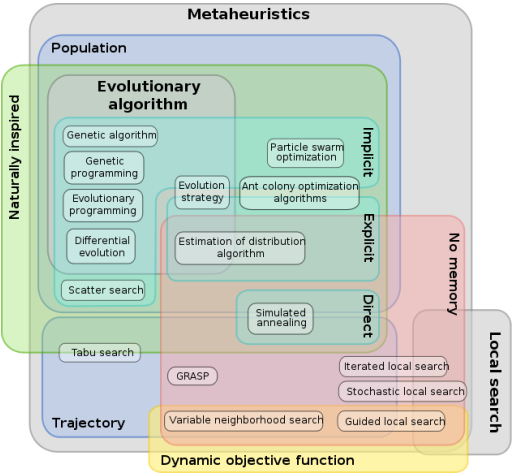
\includegraphics[]{MarcoConceptual/images/classification_mh.png} 
%\caption{Classification of Metaheuristic}\label{fig:classification-of-mh}
%\squeezeup

%TABLA (musician - > decision variables)
\squeezeup


\begin{figure}[ht]
	\centering
  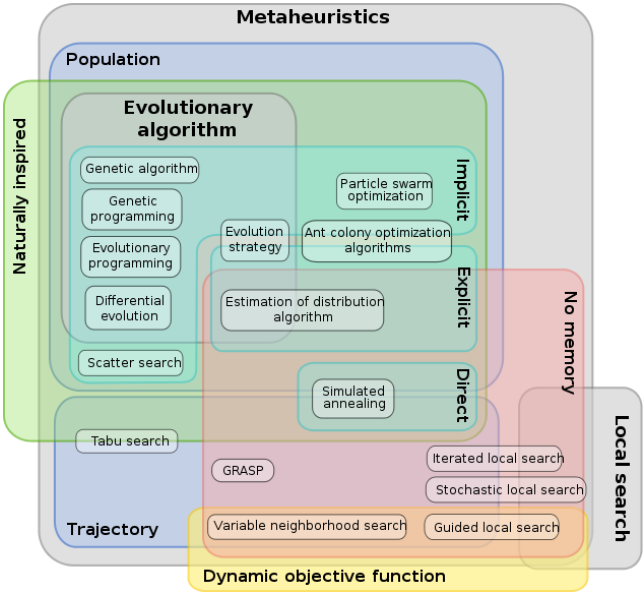
\includegraphics[width=0.55\textwidth]{MarcoTeorico/imagenes/classification_mh.png}
	\caption{Classification of Metaheuristic}\label{fig:classification-of-mh}
\end{figure}

\squeezeup


\subsubsection{Operator} 
Unitary procedure for transforming information or implement the behavior of the algrithm.

\subsubsection{Solution} 
Array of $n$ columns containing a solution for a given problem. In the binary case, the posible values are $0$ and $1$.

\subsubsection{Constrain} 
Conditions to be met to find a viable solution.

\subsubsection{Benchmark} 
Optimal set of known problem instances to validate the propose algorithm.

\subsubsection{Objective Function}  
Implements the mathematical expression representing the problem to solve. The guiding objective function is related to the goal to achieve.

\subsubsection{Fitness} 
Value resulting by applying the objective function to solution.

\subsubsection{Matrix of Costs} 
Consist of $n$ columns vector containing the cost associated with each problem variable.

\subsubsection{Optimal Value} 
Solution with the best fitness.

\subsubsection{Domain} 
Set of possible values for the variable.

\subsubsection{Matrix A} 
Matrix containing the restrictions for the given problem.

\subsubsection{RPD} 
Relative Percentage Deviation.

\subsubsection{Harmony Memory} 
Memory space which includes the population of the solution vectors.

\subsubsection{Harmony Memory Size} 
Defines the amount of harmonies that can be stored in HM.

\subsubsection{Harmony Memory Consideration Rate (HMCR)} 
In memory consideration, the value of decision variable ${x\textprime}_1$ is randomly selected from the historical values, other decision variables, $({x\textprime}_2, {x\textprime}_3,\dots,{x\textprime}_N)$ are sequentially selected in the same manner with probability where HMCR $\in$ (0,1).

\subsubsection{Pitch Adjusting Rate (PAR)} 
Each decision variable ${x\textprime}_i$ assigned a value by memory considerations is pitch adjusted with the probability of PAR where PAR $\in$ (0,1).

\squeezeup
\begin{figure}
\centering
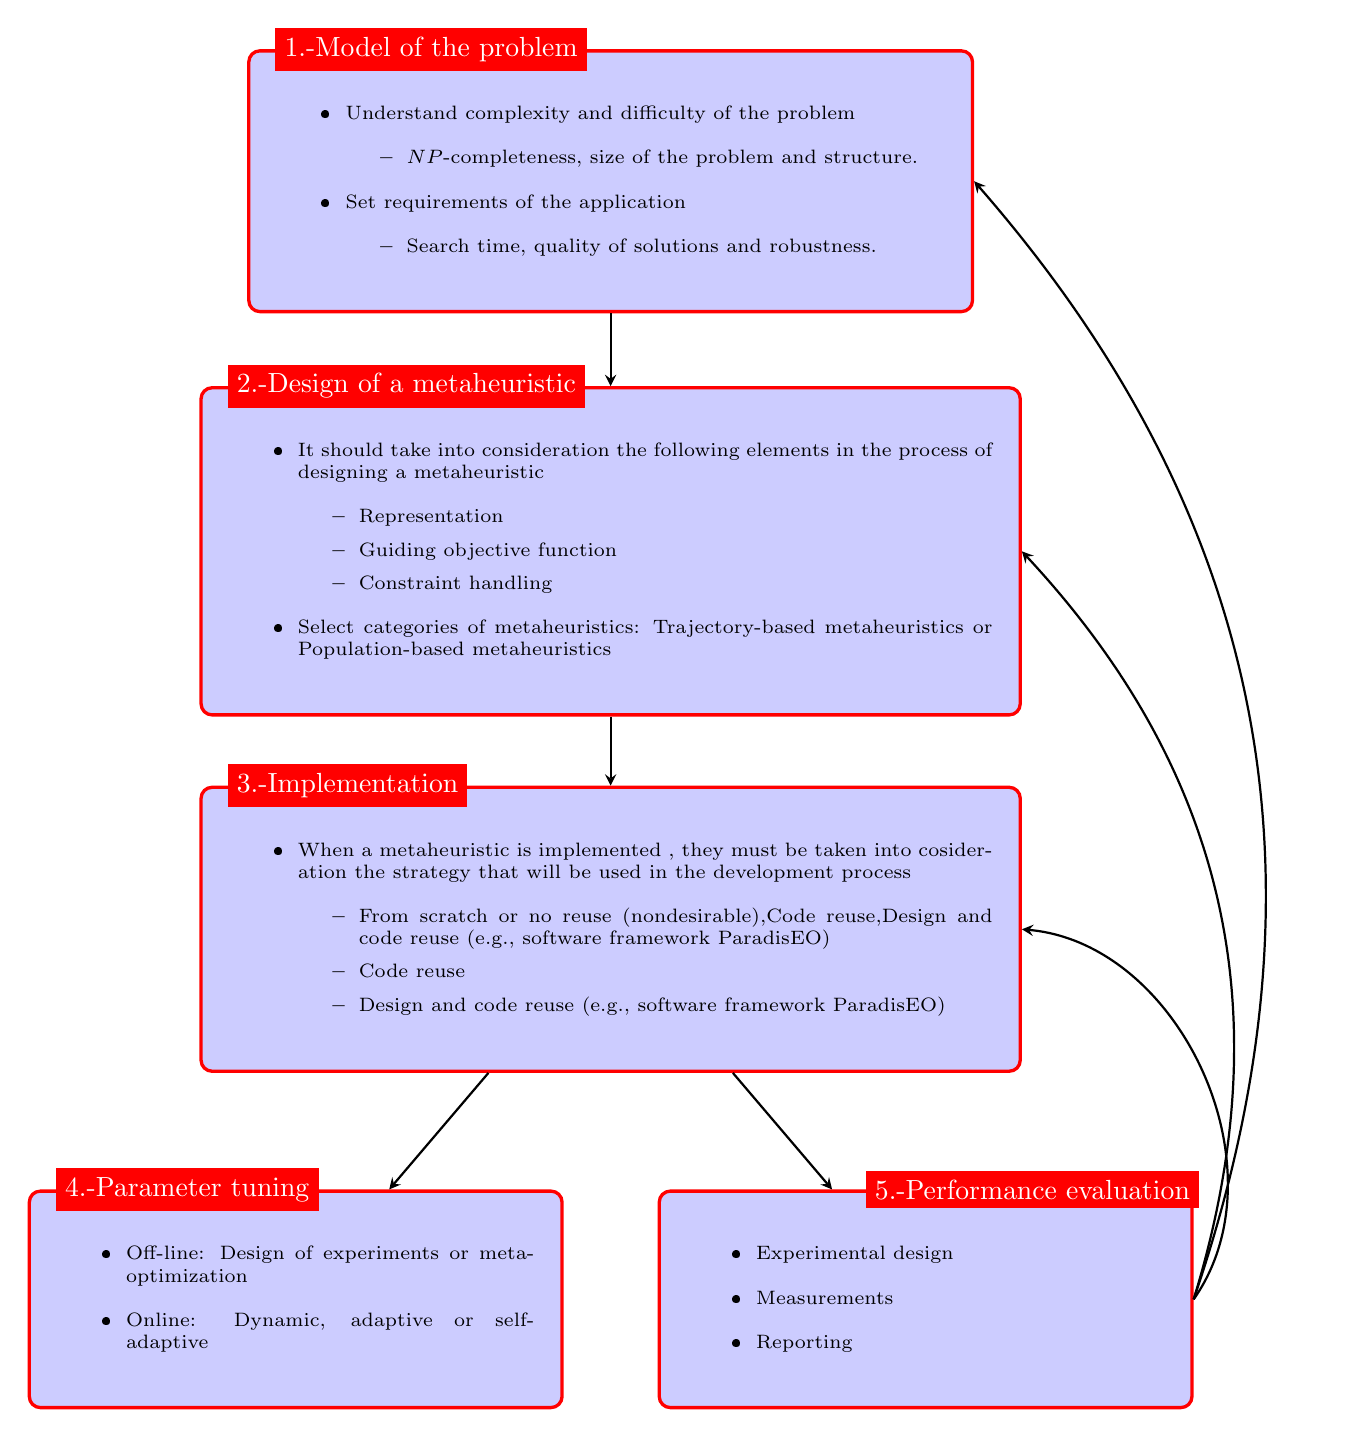
\begin{tikzpicture}[node distance=0.5cm]

%Nodo 1==============================================
\node (pro1) [mybox] {
	\begin{minipage}{0.70\textwidth}
	\scriptsize
		 \begin{itemize}
		 	\item{Understand complexity and difficulty of the problem}
			\begin{itemize}
				\item{$NP$-completeness, size of the problem and structure.}
			\end{itemize}	
			\item{Set requirements of the application}
			\begin{itemize}
				\item{Search time, quality of solutions and robustness.}
			\end{itemize}	
		 \end{itemize}
		 
	\end{minipage}
};
\node[fancytitle, right=10pt] at (pro1.north west) {1.-Model of the problem};

%Nodo 2==============================================
\node (pro2) [mybox, below of=pro1, yshift=-4.2cm] {
	\begin{minipage}{0.80\textwidth}
		\scriptsize
		 \begin{itemize}
		 	\item{It should take into consideration the following elements in the process of designing a metaheuristic}
			\begin{itemize}
				\item{Representation}
				\item{Guiding objective function}
				\item{Constraint handling}
			\end{itemize}
			\item{Select categories of metaheuristics: Trajectory-based metaheuristics or Population-based metaheuristics}
		 \end{itemize}
		 
	\end{minipage}
};
\node[fancytitle, right=10pt] at (pro2.north west) {2.-Design of a metaheuristic};

%Nodo 3============================================
\node (pro3) [mybox, below of=pro2, yshift=-4.3cm] {
	\begin{minipage}{0.80\textwidth}
		\scriptsize
		 \begin{itemize}
		 \item{When a metaheuristic is implemented , they must be taken into cosideration the strategy that will be used in the development process}
		 \begin{itemize}
		 	\item{From scratch or no reuse (nondesirable),Code reuse,Design and code reuse (e.g., software framework ParadisEO)}
			\item{Code reuse}
			\item{Design and code reuse (e.g., software framework ParadisEO)}
		 \end{itemize}
		\end{itemize}
	\end{minipage}
};
\node[fancytitle, right=10pt] at (pro3.north west) {3.-Implementation};

%Nodo 4=============================================
\node (pro4) [mybox,below of=pro3, yshift=-4.2cm, xshift=-4.0cm] {
	\begin{minipage}{0.50\textwidth}
		\scriptsize
		 \begin{itemize}
		 	\item{Off-line: Design of experiments or meta-optimization}
		 	\item{Online: Dynamic, adaptive or self-adaptive}
		 \end{itemize}
		 
	\end{minipage}
}; 
\node[fancytitle, right=10pt] at (pro4.north west) {4.-Parameter tuning};

%Nodo 5==============================================
\node (pro5) [mybox,below of=pro3, yshift=-4.2cm, xshift=4.0cm] {
	\begin{minipage}{0.50\textwidth}
		\scriptsize
		 \begin{itemize}
		 	\item{Experimental design}
			\item{Measurements}
			\item{Reporting}
		 \end{itemize}
		 
	\end{minipage}
}; 
\node[fancytitle, right=75pt] at (pro5.north west) {5.-Performance evaluation};
%==============================================
\draw [arrow] (pro1) --  (pro2);
\draw [arrow] (pro2) -- (pro3);
\draw [arrow] (pro3) -- (pro4);
\draw [arrow] (pro3) -- (pro5);
\draw [arrow] (pro5.east) to [bend right=30] (pro1.east);
\draw [arrow] (pro5.east) to [bend right=30] (pro2.east);
\draw [arrow] (pro5.east) to [bend right=60] (pro3.east);
\end{tikzpicture}
\caption{Guidelines for solving SCP.}\label{fig:GuideSolvingSCP}
\end{figure}


\subsection{Set Covering Problem}
\subsubsection{SCP formulation}
The SCP is a well-known mathematical problem, which tries to cover a set of needs at the lowest possible cost. The SCP was included in the list of 21  $\mathcal{N} \mathcal{P}$-\textit{complet} problems of Karp \cite{DBLP:books/daglib/p/Karp10}. There are many practical uses for this problem, such as: crew scheduling \cite{ref02, ref08}, location of emergency facilities \cite{ref51,Vasko198485}, production planning in industry \cite{Vasko:1987:OSI:40299.40301,ref48, ref50}, vehicle routing \cite{ref07, ref27}, ship scheduling \cite{ref26, ref13}, network attack or defense \cite{ref14}, assembly line balancing \cite{ref28, ref41}, traffic assignment in satellite communication systems \cite{ref37, ceriaetal1998}, simplifying boolean expressions \cite{ref16}, the calculation of bounds in integer programs \cite{ref18}, information retrieval \cite{ref20}, political districting \cite{ref29}, crew scheduling problems in airlines \cite{doi:10.1287/inte.27.5.68}, among others.
The SCP can be formulated as follows:

\begin{equation} \label{ec:set-covering-1}  
\mbox{Minimize} \quad Z = \sum_{j = 1}^{n} c_j x_j
\end{equation}
Subject to:
\begin{equation} \label{ec:set-covering-2} 
\sum_{j = 1}^{n} a_{ij} x_j \geq 1 \quad  \forall i \in I
\end{equation}
\begin{equation} \label{ec:set-covering-3} 
x_j \in \{0,1\} \quad  \forall j \in J 
\end{equation}	


Let $A = (a_{ij})$ be a $m \times n$ 0-1 matrix with $I = \{ 1,\dots, m\}$ and $J = \{ 1,\dots, n\}$ be the row and column sets respectively. We say that column $j$ can be cover a row $i$ if $a_{ij} = 1$. Where $c_j$ is a nonnegative value that represents the cost of selecting the column $j$ and $x_j$ is a decision variable, it can be 1 if column $j$ is selected or 0 otherwise. The objective is to find a minimum cost subset $S \subseteq J$, such that each row $i \in I$ is covered by at least one column $j \in S$. 
\vspace{0mm}\\

In the following section, we present a simple way to understand the SCP, through an example:\\

\subsubsection{SCP sample solution}
Imagine that an ambulance station can meet the needs of an geographic zone. Similarly the ambulance station can cover all the needs of the nearby areas. For example, if a station is built in Zone 1 (Figure~\ref{fig:SetCovering}) ambulance station can meet the needs of neighboring areas, that is, it could also cover: Zone 1, Zone 2, Zone 3 and Zone 4.  This can be appreciated in equation (\ref{ec:rest1}).

In this example, we must fulfill the need to cover the geographical areas defined in accordance with the restrictions.

The restriction of this case is that all areas must be covered by at least one ambulance station and the goal is to minimize the number of stations built, the cost of building a station is the same for all areas. The $x_j$ variable represents the area $j$ which is $1$ if the ambulance station is built, and will be $0$ if not. As above, it can be formulated as follows:

\squeezeup
\begin{figure}[!http]
	\begin{center}
		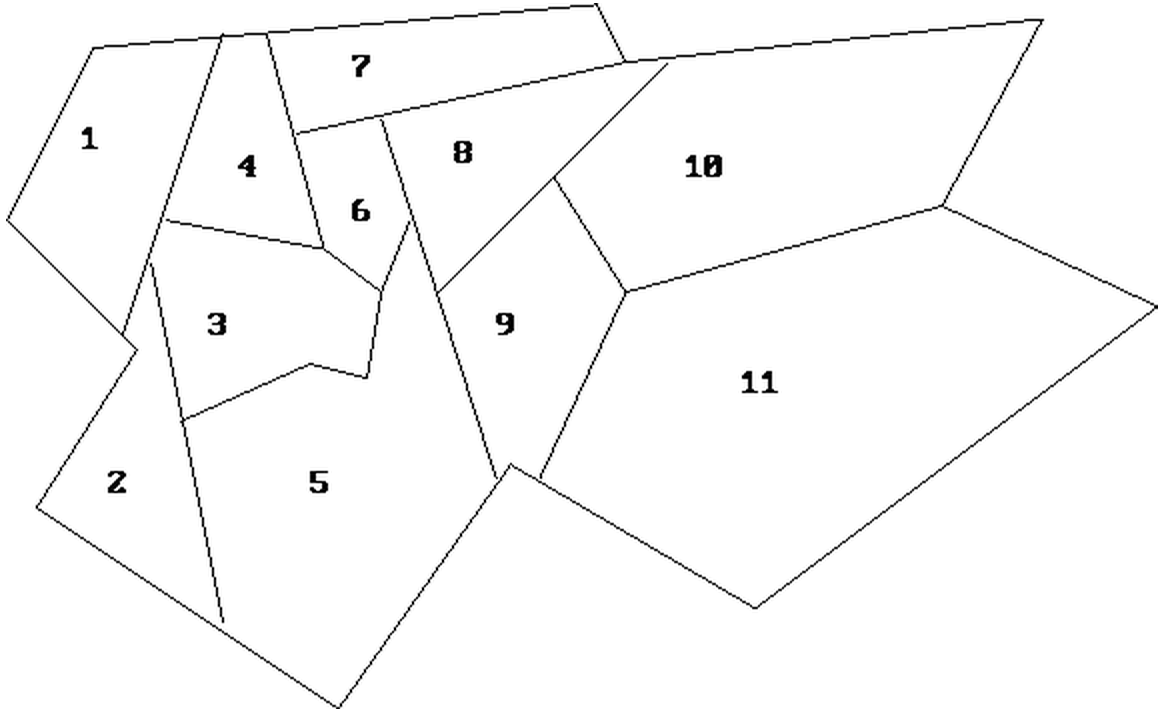
\includegraphics[width=0.8\linewidth]{Introduccion/imagenes/SetCovering.png}
		\caption{Set Covering Problem example.}\label{fig:SetCovering}
	\end{center}
\end{figure}
\squeezeup

\scriptsize
\begin{equation} \label{ec:SetCoveringExample} 
\mbox{Min} \quad c_{1}x_{1} + c_{2}x_{2} + c_{3}x_{3} + c_{4}x_{4} + c_{5}x_{5} + c_{6}x_{6} + c_{7}x_{7} + c_{8}x_{8} + c_{9}x_{9} + c_{10}x_{10} + c_{11}x_{11}
\end{equation}

Subject to:
\begin{align}
x_{1} & + & x_{2} & + & x_{3} & + & x_{4} &  &  &  &  &  &  &  &  &  &  &  &  &  &  & \geq  1 \label{ec:rest1}  \\
x_{1} & + & x_{2} & + & x_{3} &  &  & + & x_{5} &  &  &  &  &  &  &  &  &  &  &  &  & \geq  1 \\
x_{1} & + & x_{2} & + & x_{3} & + & x_{4} & + & x_{5} & + & x_{6} &  &  &  &  &  &  &  &  &  &  & \geq  1 \\
x_{1} &  &  & + & x_{3} & + & x_{4} &  &  & + & x_{6} & + & x_{7} &  &  &  &  &  &  &  &  & \geq  1 \\
& & x_{2} & + & x_{3} &  &  & + & x_{5} & + & x_{6} &  &  & + & x_{8} & + & x_{9} &  &  &  &  & \geq  1 \\
& & & & x_{3} & + & x_{4} & + & x_{5} & + & x_{6} & + & x_{7} & + & x_{8} &  &  &  &  &  &  & \geq  1 \\
& & & & & & x_{4} & & & + & x_{6} & + & x_{7} & + & x_{8} & & & & & & & \geq  1 \\
& & & & & & & & x_{5} & + & x_{6} & + & x_{7} & + & x_{8} & + & x_{9} & + & x_{10} & & & \geq  1 \\
& & & & & & & & x_{5} & & & & & + & x_{8} & + & x_{9} & + & x_{10} & + & x_{11} & \geq  1 \\
& & & & & & & & & & & & & & x_{8} & + & x_{9} & + & x_{10} & + & x_{11} & \geq  1 \\
& & & & & & & & & & & & & & & & x_{9} & + & x_{10} & + & x_{11} & \geq  1 
\end{align}
\normalsize

The first constraint (\ref{ec:rest1}) indicates that to cover zone 1, it is possible to locate a station in the same area or in the border. The following restriction is for zone 2 and so on. One possible optimal solution for this problem is to locate ambulance stations in zones 3, 8 and 9. That is, $x_{3} = x_8 = x_9 = 1$ y $x_{1} = x_{2} = x_{4} = x_{5} = x_{6} = x_{7} = x_{10} = x_{11} = 0$. As shown in (Figure~\ref{fig:SetCovering2}).

\squeezeup
\begin{figure}[!http]
	\begin{center}
		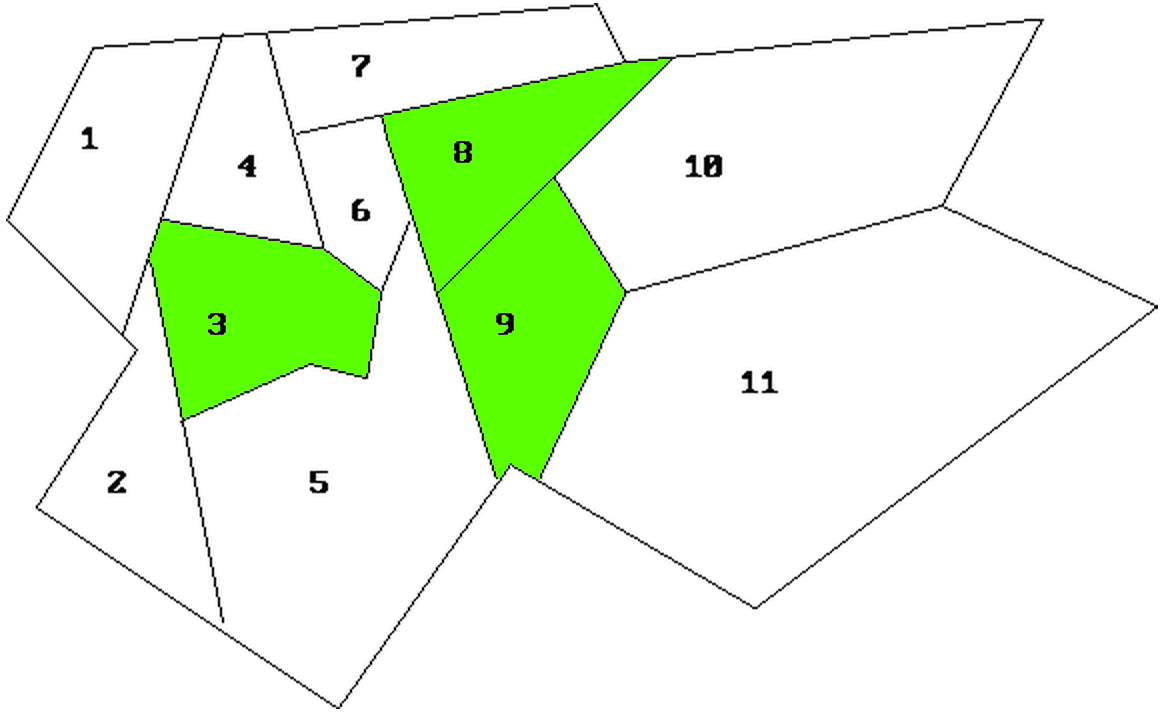
\includegraphics[width=0.8\linewidth]{Introduccion/imagenes/SetCoveringSolved.png}
		\caption{Set Covering Problem solution.}\label{fig:SetCovering2}
	\end{center}	
\end{figure}
\squeezeup

%\subsection{Unicost SCP}
%The Unicost \cite{DBLP:conf/ieaaie/Musliu06,DBLP:journals/eor/AzimiTG10} is a variation of the SCP where the cost of each decision variable is 1. This indicates that it does not matter which one is active, what matters is to comply with the restrictions.


We propose solve the SCP, with a variation metaheuristic Harmony Search (HS) called Binary Global-Best Harmony Search to obtain satisfactory solutions within a reasonable time. HS mimics the process of musical improvisation, where musicians make adjustments in tone to achieve aesthetic harmony.

\subsubsection{Harmony Search Metaheuristic}
Harmony Search (HS) is a population-based metaheuristic algorithm inspired from the musical process of searching for a perfect state of Harmony or Aesthetic Quality of a Harmony (AQH). The HS was proposed by Z. W. Geem et al.\cite{DBLP:journals/simulation/GeemKL01}.

In other words, the main idea of the HS metaheuristic is to mimic the process performed by musicians when they try to play a beautiful harmony.

For the purpose of properly understand what is looking like a good solution in this metaheuristic, we must know the meaning of AQH, this concept and others are defined below.

The AQH in an instrument it is essentially determined by its pitch (or frequency), sound quality, and amplitude (or loudness). The sound quality is mainly determined by the harmonic content that is in turn determined by the waveforms or modulations of the sound signal. However, the harmonics that it can generate will largely depend on the pitch or frequency range of the particular instrument \cite{Geem:2009:MHS:1643438}.

Different notes have different frequencies. For example, the note A  has a fundamental frequency of $f_0=440 Hz$. The fundamental frequency of each note can be seen in (Table~\ref{fig:musical_notes}). 

Given the above, it is established that a good harmony has good AQH.

The pitch of each musical instrument determines the AQH, just as the fitness function values determines the quality of the decision variables.

In the music improvisation process, all musicians sound pitches within possible range together to make one harmony.

If all pitches make a good harmony, each musician stores in his memory that experience and possibility of making a good harmony in increased next time. The same thing in optimization, the initial solution is generated randomly from decision variables within the possible range.

If the objetive function values of these decision variables is good to make promising solution, then the possibility to make a good solution is increased next time.

\begin{table}[]
\centering
\begin{tabular}{|l|l|}
\hline
\textbf{Musical Note} & \textbf{Frequency} \\ \hline
C                     & 261,625565 Hz      \\ \hline
D                     & 293,664768 Hz      \\ \hline
E                     & 329,627557 Hz      \\ \hline
F                     & 349,228231 Hz      \\ \hline
G                     & 391,995436 Hz      \\ \hline
A                     & 440,000000 Hz      \\ \hline
B                     & 493,883301 Hz      \\ \hline
\end{tabular}
\caption{HS - Musical Notes}\label{fig:musical_notes}
\end{table}


In this document, we focus on studying the classical SCP problem (equation \ref{ec:set-covering-1}), where we want minimize the cost.

\subsubsection{HS operation in depth}
In general, the procedure for HS metaheuristic, consists of the following four steps.\\ \\

\emph{Step 1: Initialization parameters} \\
The parameters required to solve the optimization problem are speci?ed in this step, an initial HM is filled with a population of  Harmony Memory Size (HMS), harmonies are generated randomly.\\ 
In addition, the parameters of HS, that is, Harmony Memory Consideration Rate (HMCR) which determines the rate of selecting the value from the memory and Pitch Adjusting Rate (PAR) determines the probability of local improvement and number of improvisations (NI) are given when the metaheuristic begins.\\ \\
\emph{Step 2: New Harmony} \\
Improvise a new harmony from the current HM.\\ \\%The details of this procedure are given in Algorithm \ref{alg:newHarmonyGreedy}.
\emph{Step 3: Replace worst Harmony in HM} \\
If the new generated harmony is better than the worst one in HM, then replace the worst harmony with the new one; otherwise, go to the next step. \\ \\
\emph{Step 4: Check the stop criteria} \\
If a stopping criterion is not satisfied, go to Step 2.

%TABLA (musician - > decision variables)
\squeezeup
\begin{table}[]
\centering
\begin{tabular}{|m{3.5cm}|m{8cm}|}
\hline
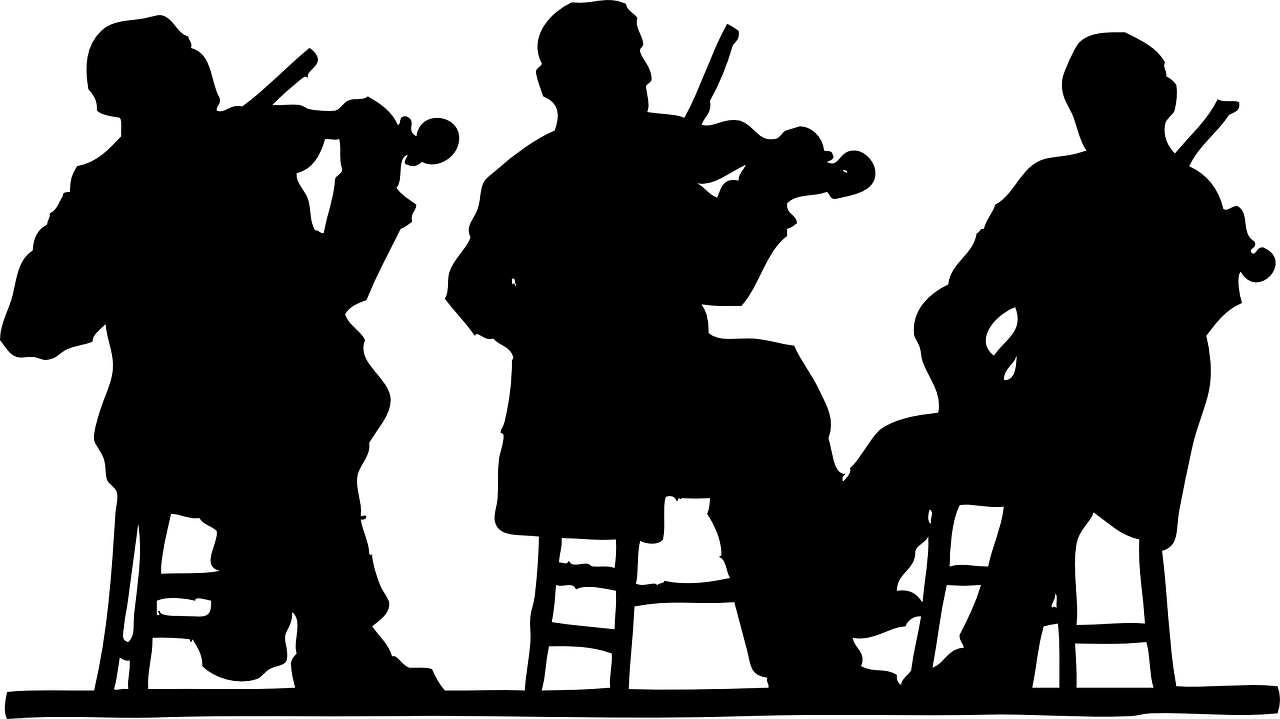
\includegraphics[width=30mm,scale=0.05]{MarcoTeorico/imagenes/musicos.png} & 
Each musician represents a decision variable,
according to the example shown, there would be 11 musicians, 	
since there are 11 decision variables $x_1\dots x_{11}$. \\ \hline
\end{tabular}
\caption{HS components - Musician}\label{fig:harmony_process_musician}
\end{table}
\squeezeup

%--VIOLIN (Instrument Pitch Range - > Range Value of decision variable)
\begin{table}[]
\centering
\begin{tabular}{|m{3.5cm}|m{8cm}|}
\hline
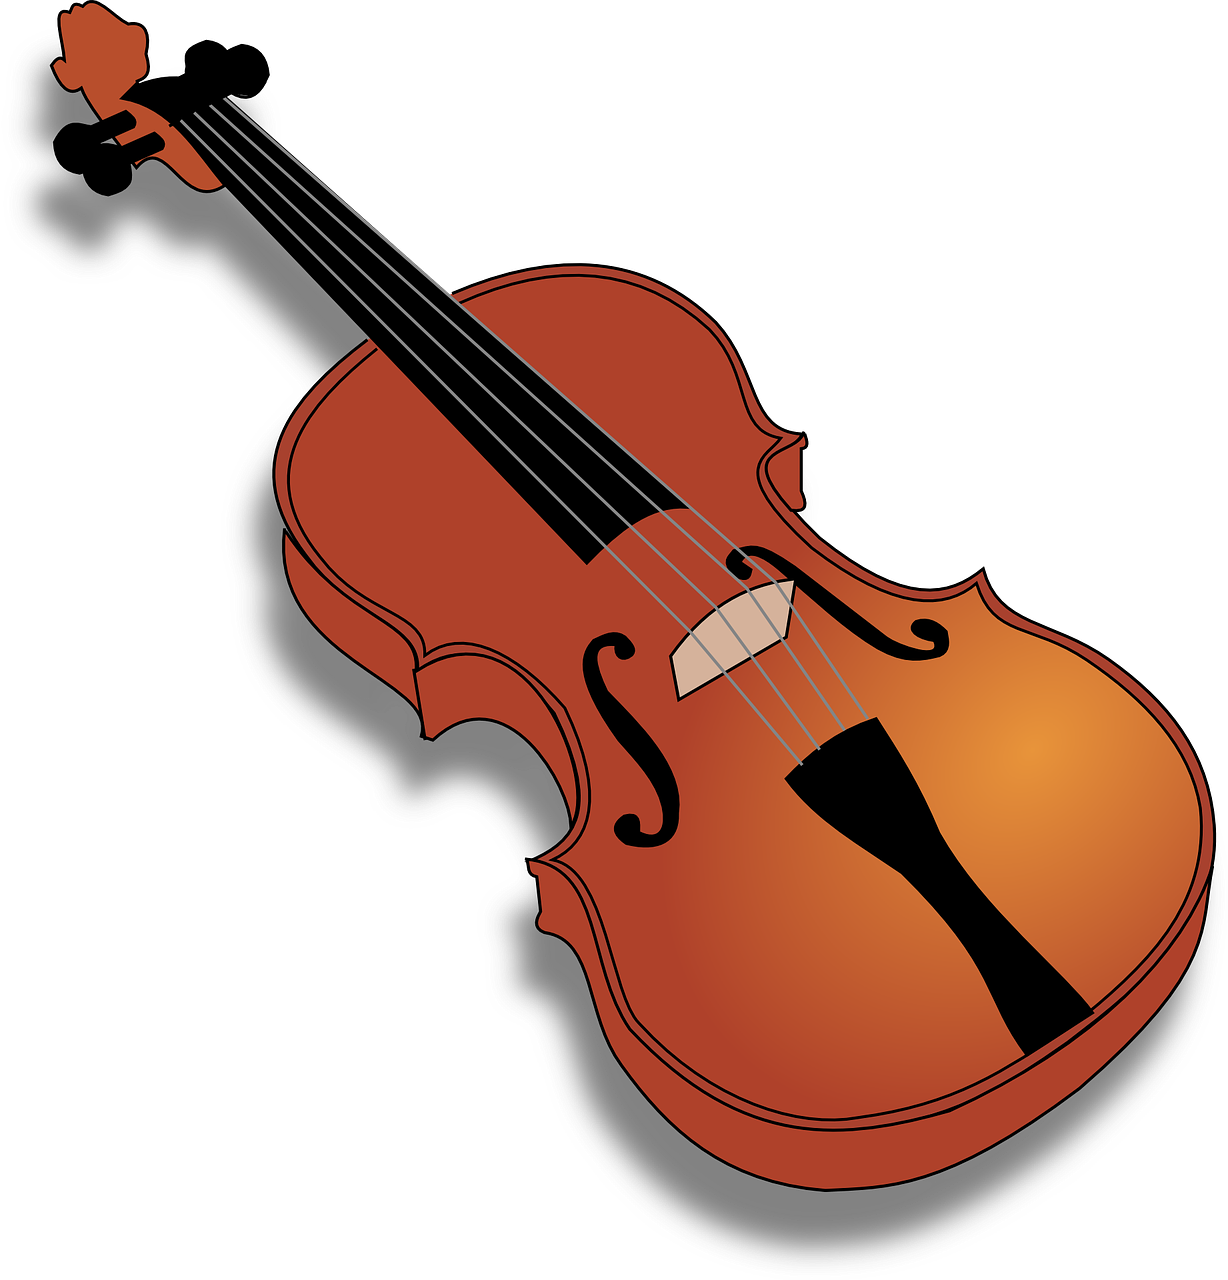
\includegraphics[width=15mm,scale=0.02]{MarcoTeorico/imagenes/violin.png} & The pitch range of the instrument represents the range of values that can take a decision variable. Given the nature of the problem, the possible values are ${\{0,1\}}$ \\  \hline\end{tabular}
\caption{HS components - Pitch range}\label{fig:harmony_process_pitch_range}
\end{table}


%--NOTA MUSICAL (Armonia -> Solucion)
\begin{table}[]
\centering
\begin{tabular}{|m{3.5cm}|m{8cm}|}
\hline

\includegraphics[width=15mm,scale=0.0005]{MarcoTeorico/imagenes/nota.png} & Musical harmony at a certain time, corresponds to a solution at a certain iteration.\\ \hline

\end{tabular}
\caption{HS components - Solution}\label{fig:harmony_process_solution}
\end{table}


% CALIDAD ESTETICA (Calidad de la armonia -> Calidad de la soluci�n)
\begin{table}[]
\centering
\begin{tabular}{|m{3.5cm}|m{8cm}|}
\hline
%$f=440\times2^{{(p_n-{69})}/12}$ & Aesthetics audience, judges whether harmony is good or not.� In the problem it refers to the objective function. \\ \hline


\includegraphics[width=30mm,scale=0.02]{MarcoTeorico/imagenes/audience.png} & Aesthetics audience, judges whether harmony is good or not.� In the problem it refers to the objective function.\\ \hline

\end{tabular}
\caption{HS components - Aesthetics audience}\label{fig:harmony_process_aesthetics}
\end{table}

%FIN TABLAS

\subsubsection{Global-Best Harmony Search Metaheuristic}
To further improve the convergence performance of HS and overcome some shortcomings of HS, a new variant of HS, called  Global-Best Harmony Search (GHS), was proposed by Omran and Mahdavi \cite{DBLP:journals/amc/OmranM08}. 
First, the GHS dynamically updates parameter PAR according to equation (\ref{ec:PAR-T}):

\begin{equation} \label{ec:PAR-T}
PAR(t) = PAR_{min}+\frac{PAR_{max} - PAR_{min}}{NI}t
\end{equation}

where $PAR(t)$ represents the pitch adjusting rate at generation $t$, $PAR_{min}$ and $PAR_{max}$  are the minimum and maximum adjusting rate, respectively.
The parameter $t$ is the iterative variable, and parameter $NI$ is the number of improvisations.


\subsubsection{Binary Global-Best Harmony Search Metaheuristic}

The HS is good at identifying the high performance regions of the solution space in a reasonable time, but poor at performing local search \cite{DBLP:journals/eswa/XiangALHZ14}. Namely, there is imbalance between the exploration and the exploitation of HS. Furthermore, HS designed for continuous space cannot be directly used to solve discrete combinatorial optimization problems.

In order to overcome the drawbacks of HS, a novel binary global-best harmony search (BGHS) is designed for binary optimization problems.

Owing to better performance of GHS, some modifications to GHS are introduced to further enhance the convergence performance of GHS. Then a novel binary coded GHS, a two-phase repair operator, and a greedy selection mechanism are integrated into the BGHS. And they are described in detail as follows.



.
.
.
.

 
























  \newpage
  
    \section{Algorithm implementation}\label{sec:algImplementation}
  \subsection{Implementation architecture}
The implementation of the algorithm was developed using the Python programming language which allows work quickly and integrate systems more effectively.
As data persistence, a MySql relational database was used, although log files were also used. All of the above was mounted on an instance of the free Amazon layer, specifically EC2 - Ubuntu GNU/Linux.
%------------------------
As a source code control system, GIT was used, which allowed to maintain a control of local source code for both the developed algorithm and the documentation associated to this thesis. Constant replicas were performed against a GIT cloud repository, specifically GITHUB.
 
\subsection{Binary Global-Best Harmony Search Metaheuristic}
The parameters presented below were the result of exhaustive tests and multiple executions that allowed to probe beyond the random components a correct behavior for metaheuristics, that is to say, presenting a higher degree of effectiveness compared to other metaheuristics.

\subsubsection{Improvising a New Harmony}
The process begins with the generation of an initial population of harmonies that are vectors composed of binary digits $d$, until the amount defined by the HMS. All harmonies are repaired after being created through two-phase repair operator (Algorithm \ref{alg:addAndDrop}).\\

Then in a repetition of the process that is called improvisation new harmonies are created. The number of improvisations is denoted by $NI$. As the harmonies are created, the two-phase operator ADD and DROP is applied to make the harmonies feasible. Once the harmonies are repaired and meet the constraints defined in the  Matrix $A$ for the SCP, the best and worst harmony, denoted by $x_ {best}$ and $x_ {worst}$, respectively, are stored. Additionally a greedy selection mechanism are integrated into the BGBHS. The greedy operation is based on the idea that the item with higher profit density ratio should be used first. And the profit density ratio can be calculated by the equation (\ref{ec:mu_j}): 

\begin{equation} \label{ec:mu_j} 
\mu_{j}={\frac{1}{c_j}}
\end{equation}	

The detail of the behavior of the metaheuristics can be reviewed in the flow chart (Figure \ref{dia:FlowBGBHS})	.

%------------------------------Diagrama de HS
\begin{figure}[]
\centering
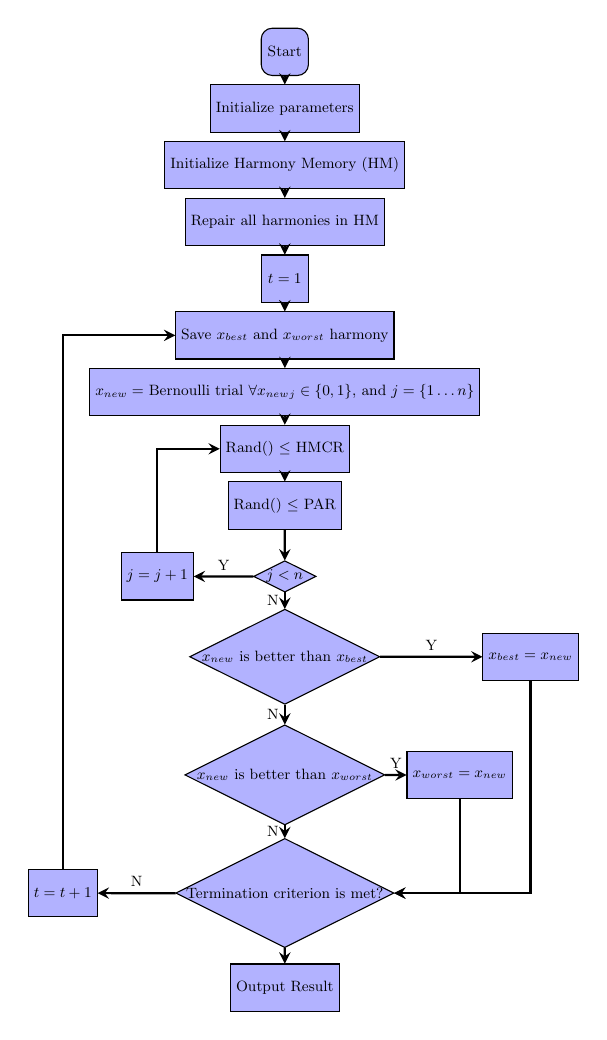
\begin{tikzpicture}[align = flush center, font = \small, node distance = 12mm, scale=0.6, every node/.style={scale=0.6}] %[node distance = 15mm, auto]
\node (start) [startstop] {Start};
\node (pro1) [process, below of=start] {Initialize parameters};
\node (pro2) [process, below of=pro1] {Initialize Harmony Memory (HM)};
\node (pro3) [process, below of=pro2] {Repair all harmonies in HM};
\node (pro4) [process, below of=pro3] {$t=1$};
\node (pro5) [process, below of=pro4] {Save $x_{best}$ and $x_{worst}$ harmony};
\node (proB) [process, below of=pro5]{$x_{new} = $ Bernoulli trial \smallskip $\forall {x_{new}}_j \in \{0,1\}$, and $j=\{1 \dots n\}$};
\node (pro6) [process, below of=proB] {Rand() $\leq$ HMCR};
\node (pro7) [process, below of=pro6] {Rand() $\leq$ PAR};
\node (pro8) [decision, below of=pro7] {$j < n$};
\node (pro9) [process, left of=pro8, xshift=-1.5cm] {$j = j + 1$};
\node (pro10) [decision, below of=pro8, yshift=-0.2cm] {$x_{new}$ is better than $x_{best}$};
\node (pro11) [process, right of=pro10, xshift=4.0cm] {$x_{best} = x_{new}$};
\node (pro12) [decision, below of=pro10, yshift=-1.0cm] {$x_{new}$ is better than $x_{worst}$};
\node (pro13) [process, right of=pro12, xshift=2.5cm] {$x_{worst} = x_{new}$};
\node (pro14) [decision, below of=pro12, yshift=-1.0cm] {Termination criterion is met?};
\node (pro15) [process, left of=pro14, xshift=-3.5cm] {$t=t+1$};
\node (pro16) [process, below of=pro14, yshift=-0.8cm] {Output Result};

%---------------------------------ARROWS
\draw [arrow] (start) -- (pro1);
\draw [arrow] (pro1) -- (pro2);
\draw [arrow] (pro2) -- (pro3);
\draw [arrow] (pro3) -- (pro4);
\draw [arrow] (pro4) -- (pro5);
\draw [arrow] (pro5) -- (proB);
\draw [arrow] (proB) -- (pro6);
\draw [arrow] (pro6) -- (pro7);
\draw [arrow] (pro7) -- (pro8);
\draw [arrow] (pro8) -- (pro9) node [midway, above] {Y};
\draw [arrow] (pro9) |- (pro6);
\draw [arrow] (pro8) -- (pro10) node [midway, left] {N};
\draw [arrow] (pro10) -- (pro11) node [midway, above] {Y};
\draw [arrow] (pro10) -- (pro12) node [midway, left] {N};
\draw [arrow] (pro12) -- (pro13) node [midway, above] {Y};
\draw [arrow] (pro12) -- (pro14) node [midway, left] {N};
\draw [arrow] (pro14) -- (pro15) node [midway, above] {N};
\draw [arrow] (pro15) |- (pro5);
\draw [arrow] (pro11) |- (pro14) ;
\draw [arrow] (pro13) |- (pro14) ;
\draw [arrow] (pro14) -- (pro16) ;

\end{tikzpicture}
\caption{Flowchart of BGBHS algorithm.}\label{dia:FlowBGBHS}
\end{figure}
%------------------------------END Diagrama de HS

The HS is good at identifying the high performance regions of the solution space in a reasonable time, but poor at performing local search \cite{DBLP:journals/eswa/XiangALHZ14}. Namely, there is an unbalance between the exploration and the exploitation. 
 
To solve the problem of local exploitation, we propose a variable parameter for the Bernoulli probability $p$ in initial population, which starts from one and decreases with each iteration, tending to zero, presenting a behavior according to the equation (\ref{ec:variable_p}):

\begin{equation} \label{ec:variable_p} 
p(t) = \frac{t}{t+1}
\end{equation}	

The graph of the function can be seen in the figure \ref{fig:pvalue}.\\

\begin{figure}[H]
\centering
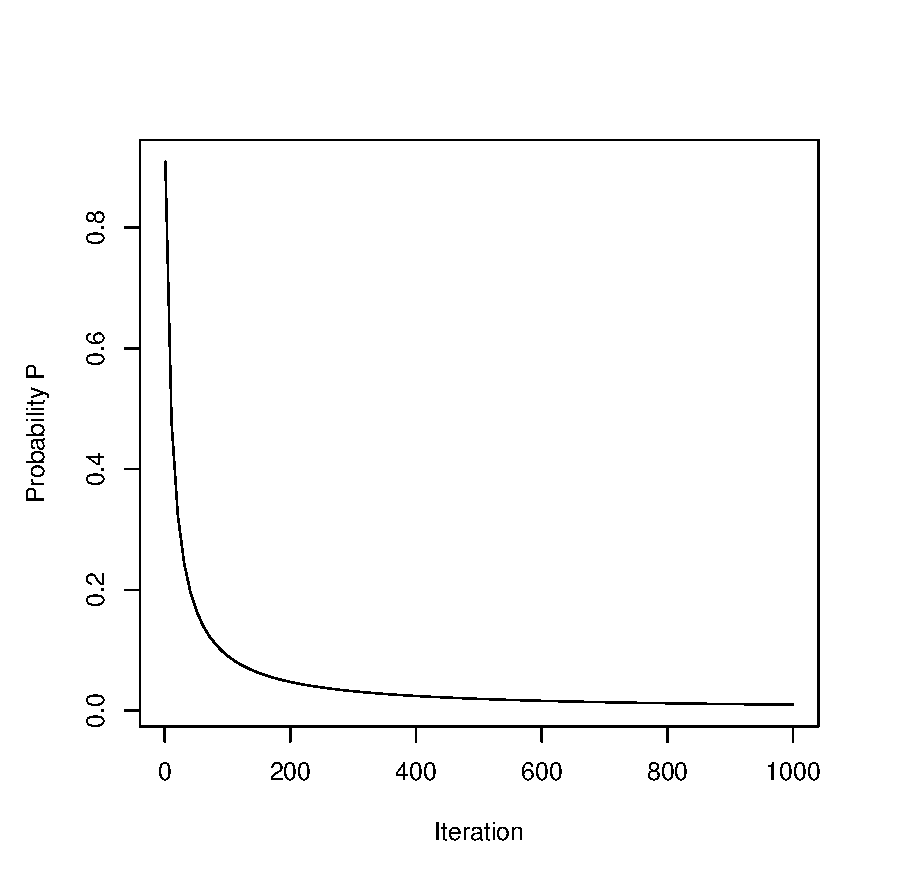
\includegraphics[scale=.35]{Implementacion/img/p_bernoulli.eps}
\caption{$p$ value over iteration}
\label{fig:pvalue}
\end{figure}

This procedure will allow solutions in a first instance to have more variables activated and as the iterations pass, the probability that a variable is activated will be closed to zero, in this way the initial population will have a wider range of solutions allowing to improve the balance between exploitation and exploration.

The initial population in BGBHS is generated randomly using a Bernoulli process. In probability and statistics, a Bernoulli process is a finite or infinite sequence of binary random variables $x_1$, $x_2$, $x_3$,\dots,$x_n$  $\forall x_i \in \{0,1\}$ ~ and ~ $i=\{1,\dots, n\}$, so it is a discrete-time stochastic process that takes only two values, success (equation \ref{ec:bernoullie_p}) or failure (equation \ref{ec:bernoullie_p-1}), given the probability $p$.

\begin{equation} \label{ec:bernoullie_p} 
P(x_i=1) = P(\text{success at the $i$-th trial}) = p 
\end{equation}	

\begin{equation} \label{ec:bernoullie_p-1} 
P(x_i=0) = P(\text{failure at the $i$-th trial}) = 1-p
\end{equation}	

Specifically, for each decision variable of an initial harmony vector, a number within is generated randomly. If the value of the number is less than $p$, the corresponding variable takes 0; otherwise it takes 1. In this way, a set of HMS harmonies will be generated randomly. All the harmonies generated by this process are probably not feasible, only through the repair operator ADD and DROP become feasible. This means that for each harmony generated, the operator must be applied to comply with the restrictions.

\subsubsection{Two-Phase Repair Operator: ADD and DROP}\label{subAddAndDrop}
New generated harmony vector needs to be repaired under two cases. One is that the harmony vector violates the constraints. The other corresponds to inactivate the most expensive columns, maintaining the feasibility of the solution. Hence, the repair operator consists of two phases. The first phase, called ADD, is responsible for repairing a harmony vector violating the constraint. The second phase, named DROP, is applied to remove any redundant column such that by removing it from the solution, the solution still remains feasible. The detail of the operation can be reviewed in the Algorithm \ref{alg:addAndDrop}.

%------------------------------Fase ADD y DROP:
\begin{algorithm}
\begin{algorithmic}[1]
 \STATE //ADD Phase
\STATE $M \gets 1,2,\ldots, m$
\STATE $A_i \sum_{j=1}^{n} a_{ij}x_{j}, i \in M$
\FOR{$j \gets 1$ \TO $n$} {
	\IF{$x_j = 0$ and $\exists i \in M, A_i < 1$ } {
		\STATE $x_j \gets 1$
		\STATE $A_i \gets A_i + a_{ij}$
	}\ENDIF
} \ENDFOR

\STATE //DROP Phase
\FOR{$j \gets n$ \TO $1$}{
	\IF{$x_j = 1$ and $\exists i \in M, A_i - a_{ij} \geq 1$ } {
		\STATE $x_j \gets 0$
		\STATE $A_i \gets A_i - a_{ij}$
	}\ENDIF
} \ENDFOR

\caption{Repair operator ADD and DROP}\label{alg:addAndDrop}
\end{algorithmic}
\end{algorithm}


%------------------------------nueva_armonia_agresiva():

  \newpage

    \section{Proposed improvements}\label{sec:propImprovements}
  improvements.tex
  \newpage

  \section{Experimental results}\label{sec:Resultados}
  Resultados


%---------------------------------------------SCP41
%!htb
\begin{figure}[]
\centering
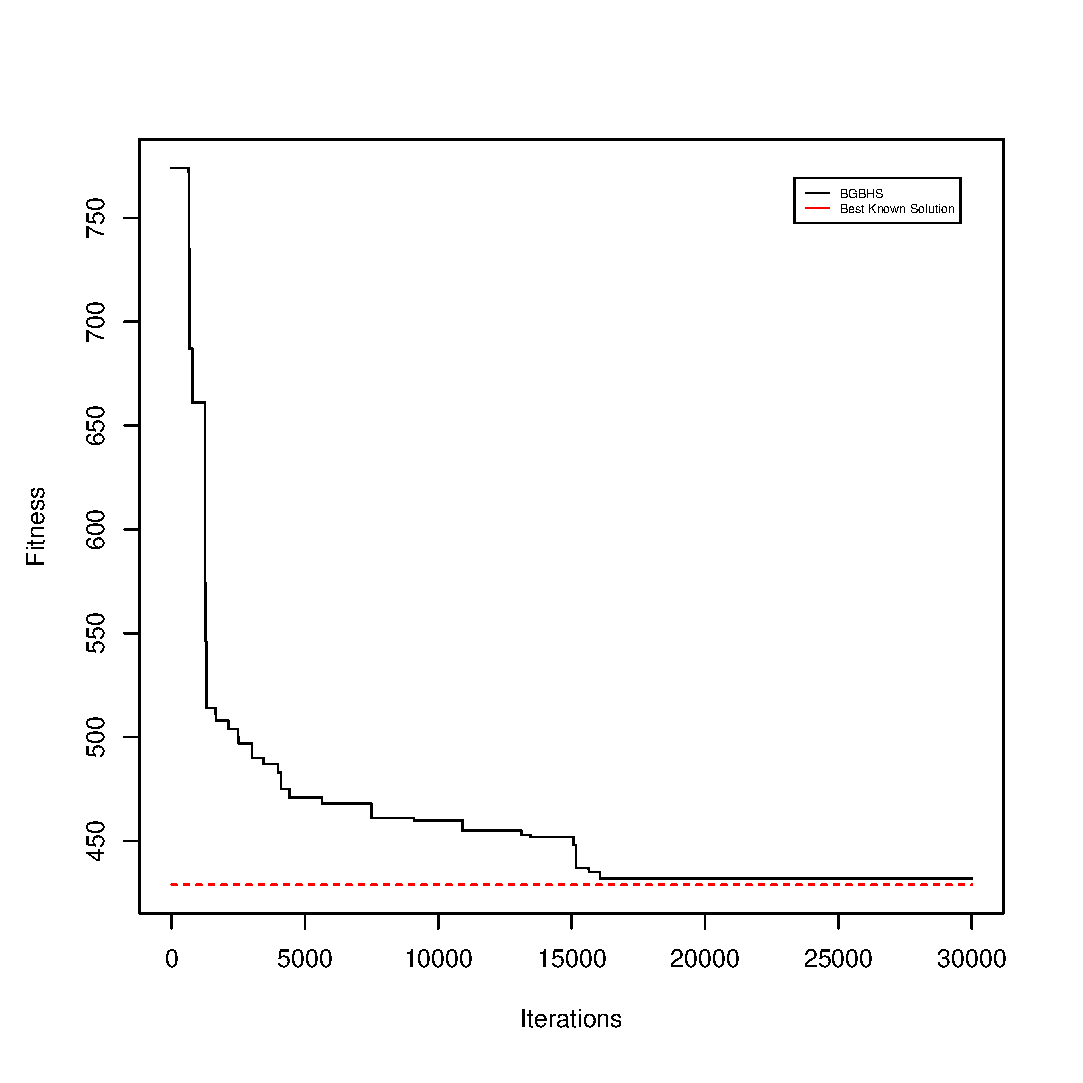
\includegraphics[scale=.45]{Resultados/scp41.eps}
\caption{Instance 4.1.}
\label{fig:Instance.4.1}
\end{figure}


%---------------------------------------------SCP42
\begin{figure}[]
\centering
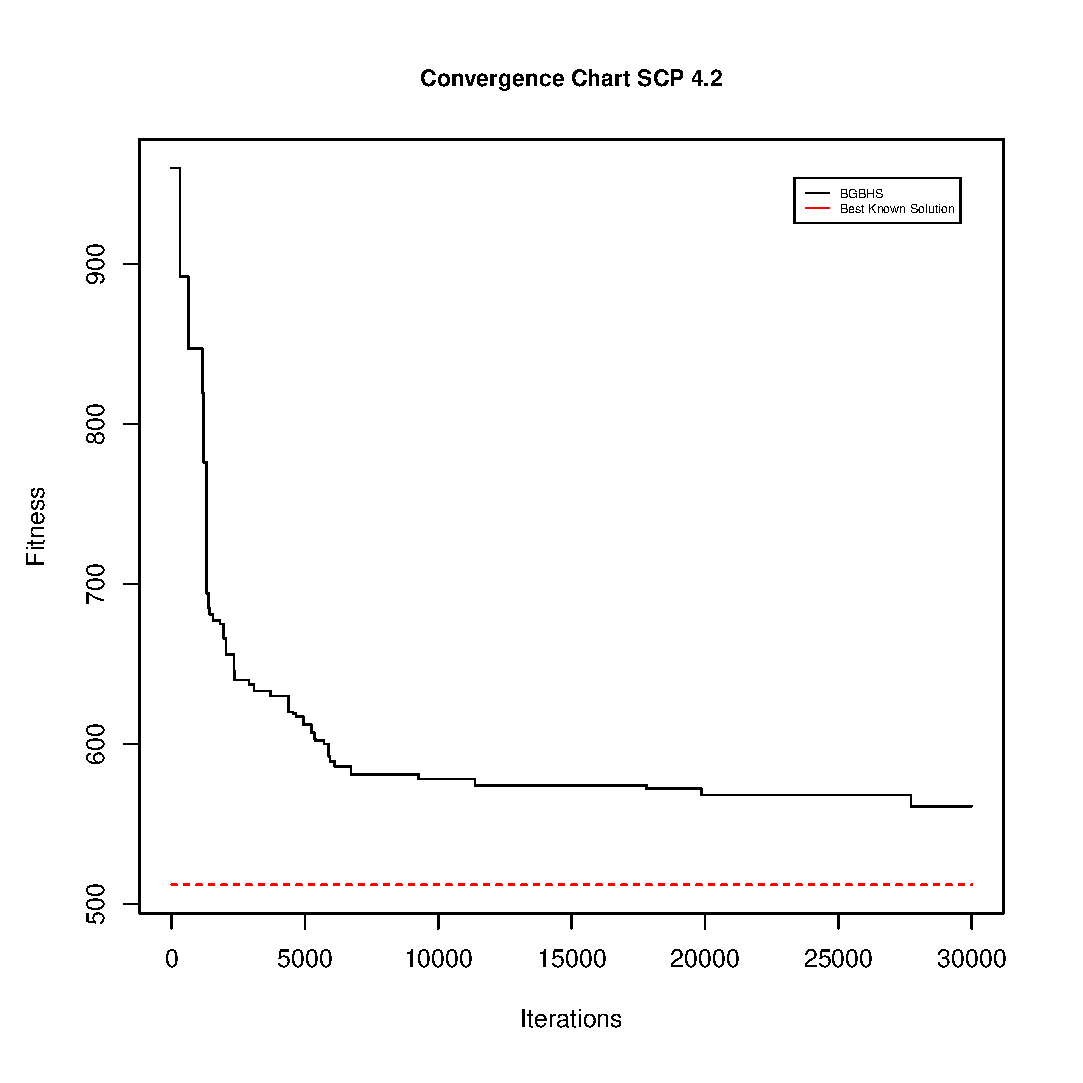
\includegraphics[scale=.45]{Resultados/scp42.eps}
\caption{Instance 4.2.}
\label{fig:Instance.4.2}
\end{figure}

%Limpieza de objetos, para liberar memoria.
\clearpage

%---------------------------------------------SCP43
\begin{figure}[]
\centering
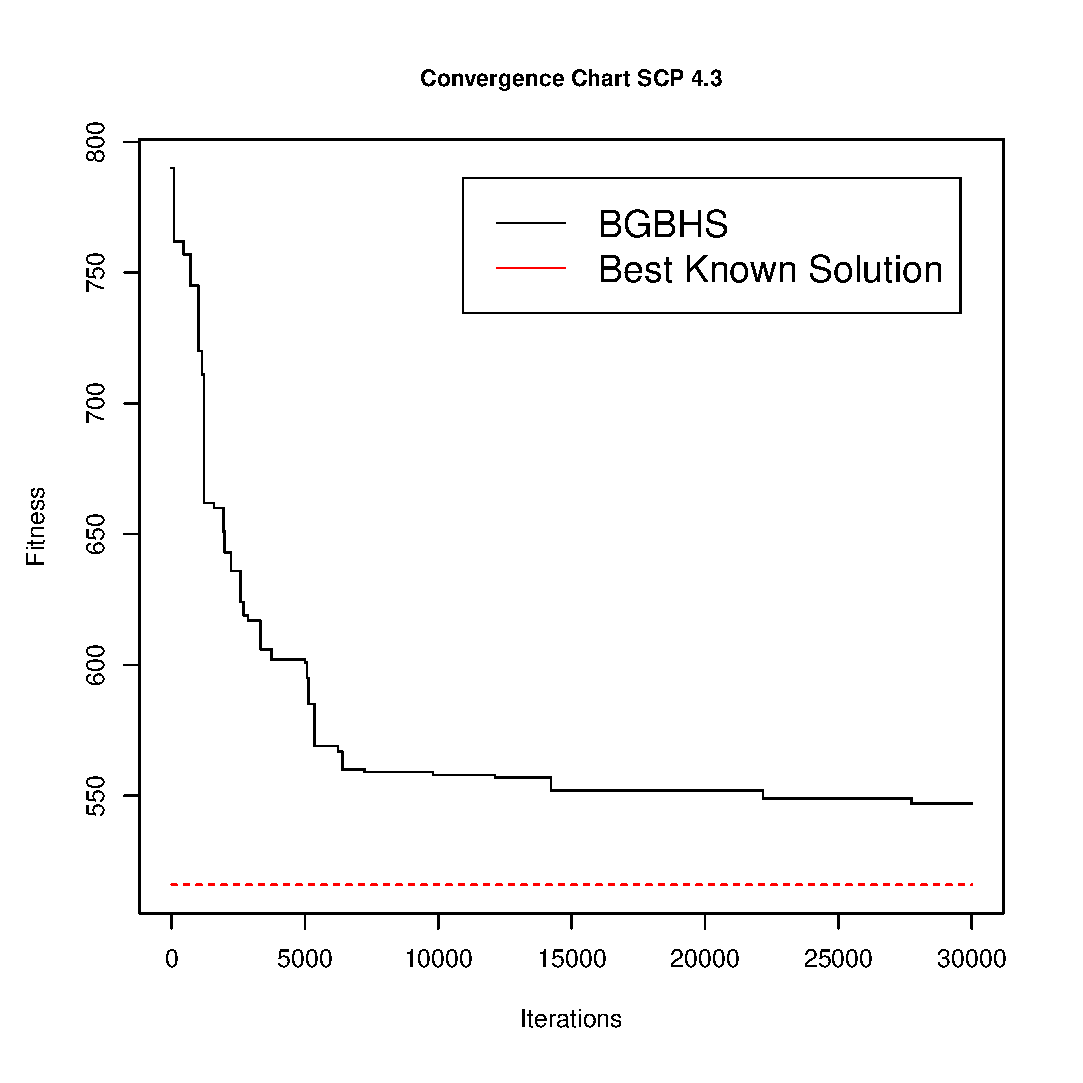
\includegraphics[scale=.5]{Resultados/scp43.eps}
\caption{Instance 4.3.}
\label{fig:Instance.4.3}
\end{figure}

%---------------------------------------------SCP44
\begin{figure}[]
\centering
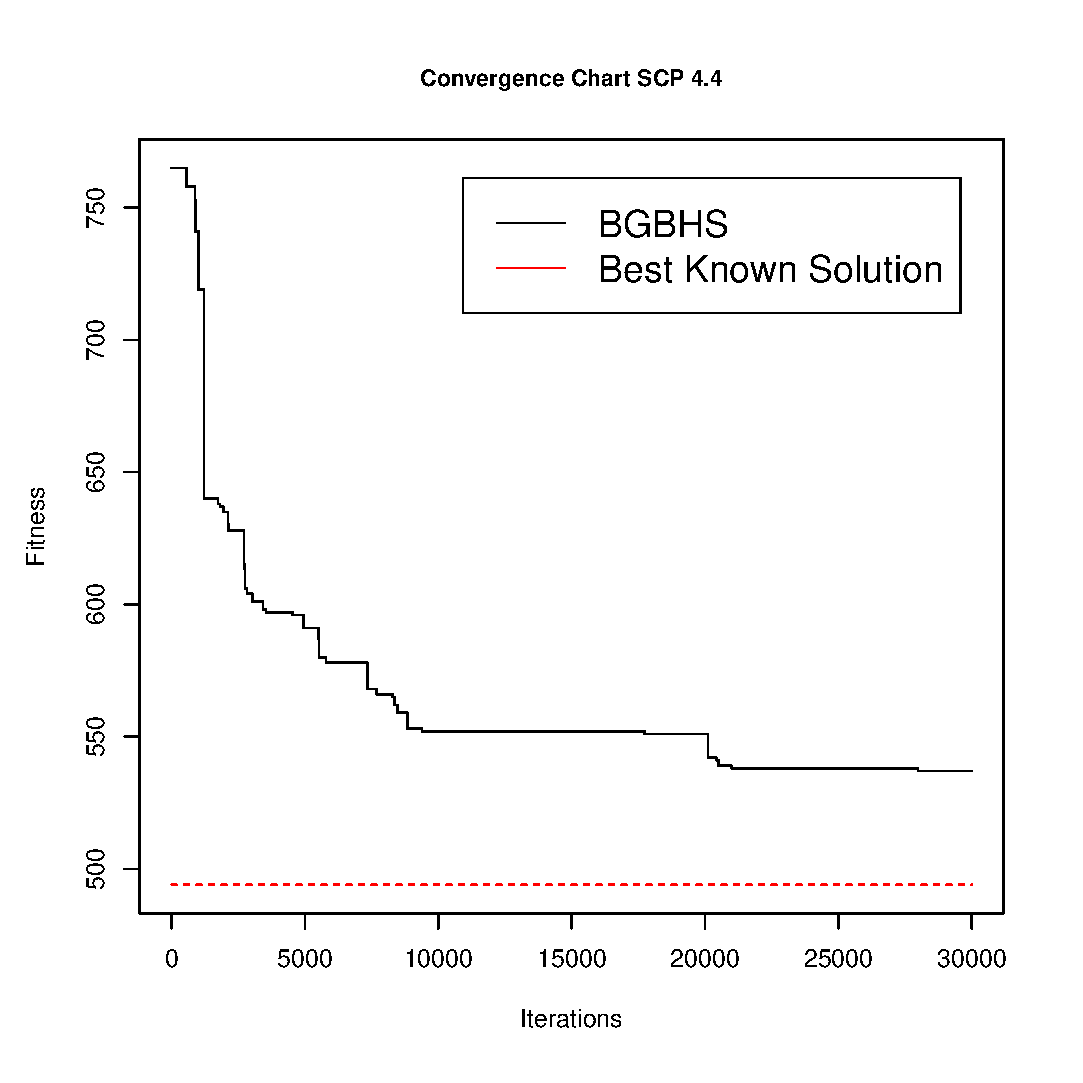
\includegraphics[scale=.45]{Resultados/scp44.eps}
\caption{Instance 4.4.}
\label{fig:Instance.4.4}
\end{figure}

%---------------------------------------------SCP45
\begin{figure}[]
\centering
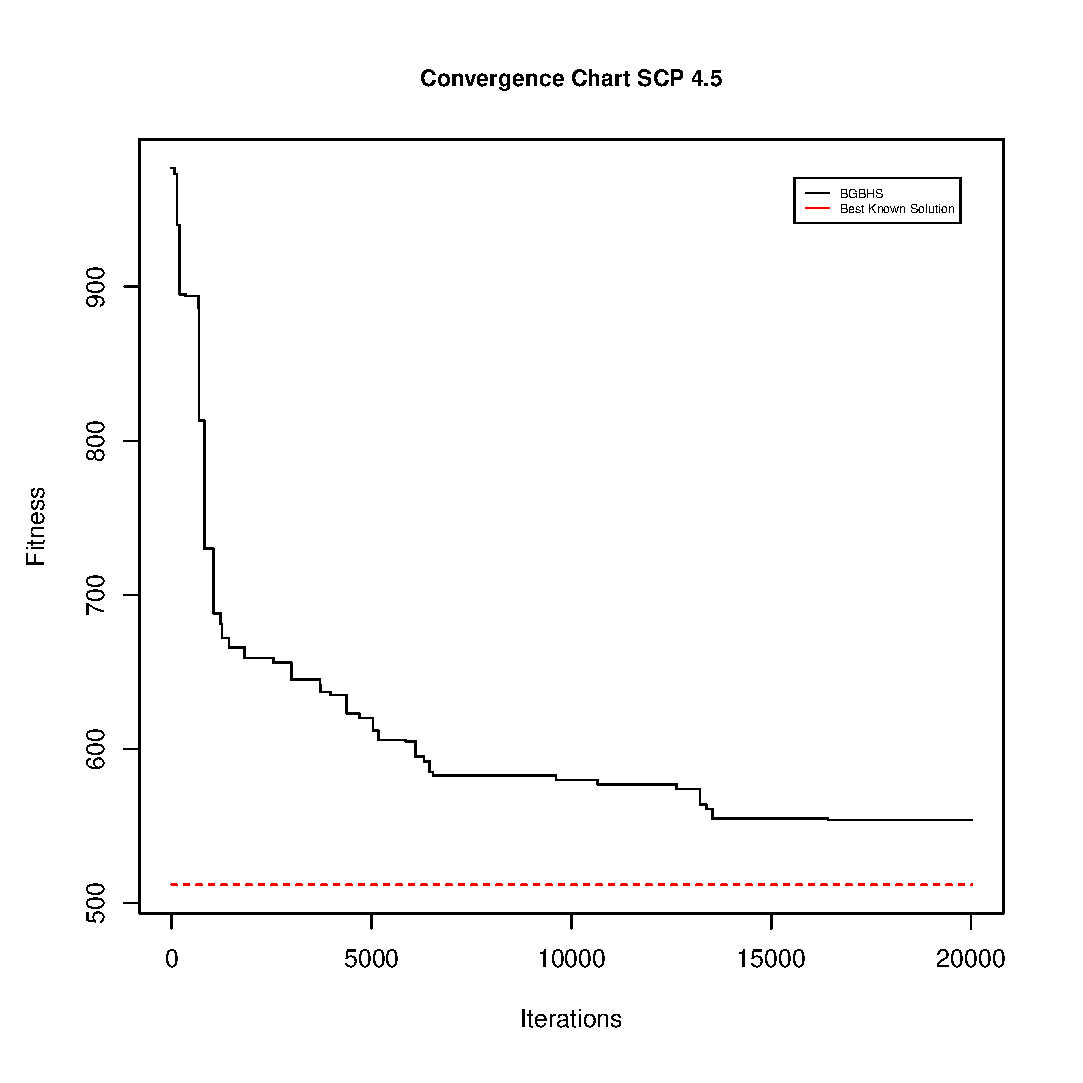
\includegraphics[scale=.45]{Resultados/scp45.eps}
\caption{Instance 4.5.}
\label{fig:Instance.4.5}
\end{figure}

%---------------------------------------------SCP46
\begin{figure}[]
\centering
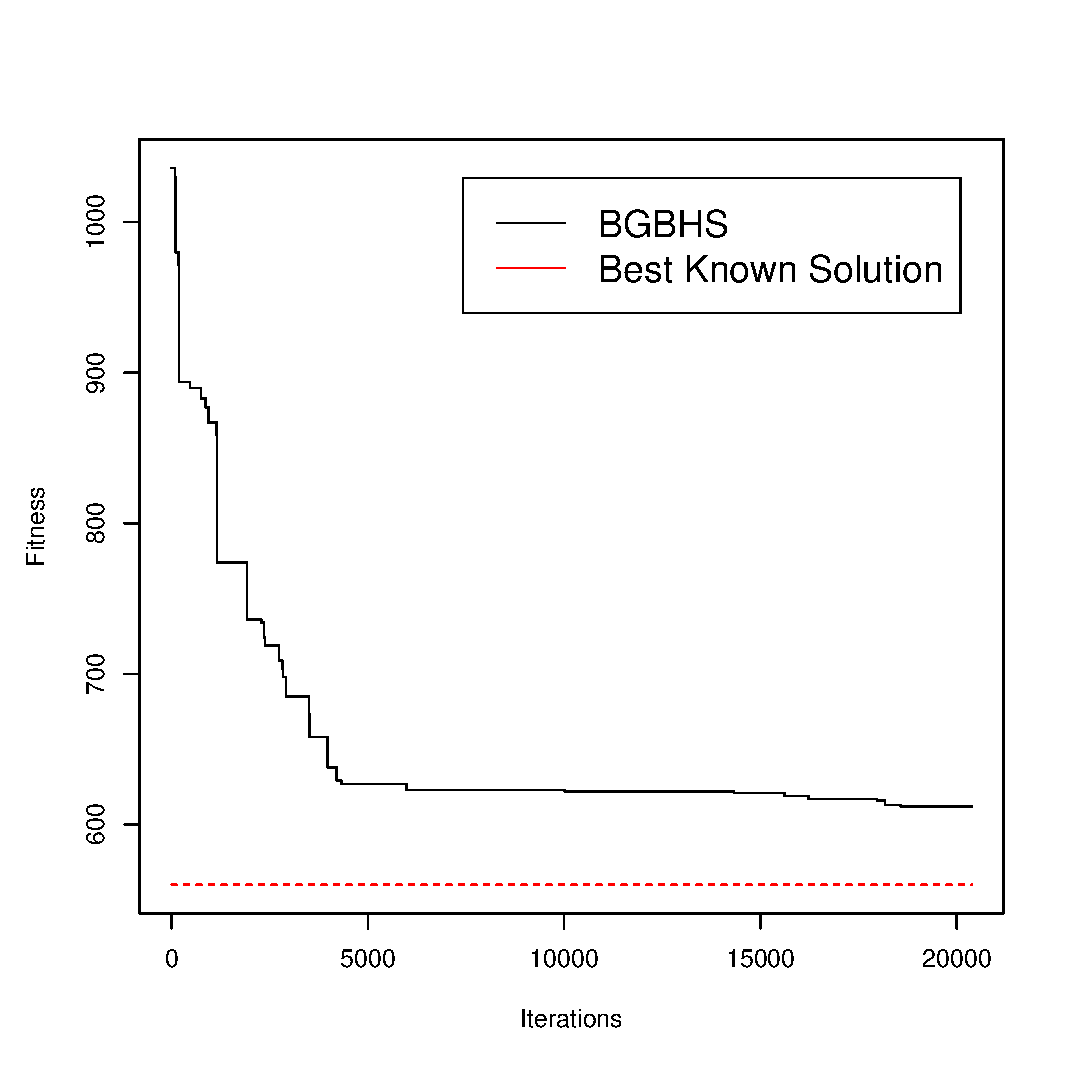
\includegraphics[scale=.45]{Resultados/scp46.eps}
\caption{Instance 4.6.}
\label{fig:Instance.4.6}
\end{figure}

%---------------------------------------------SCP47
\begin{figure}[]
\centering
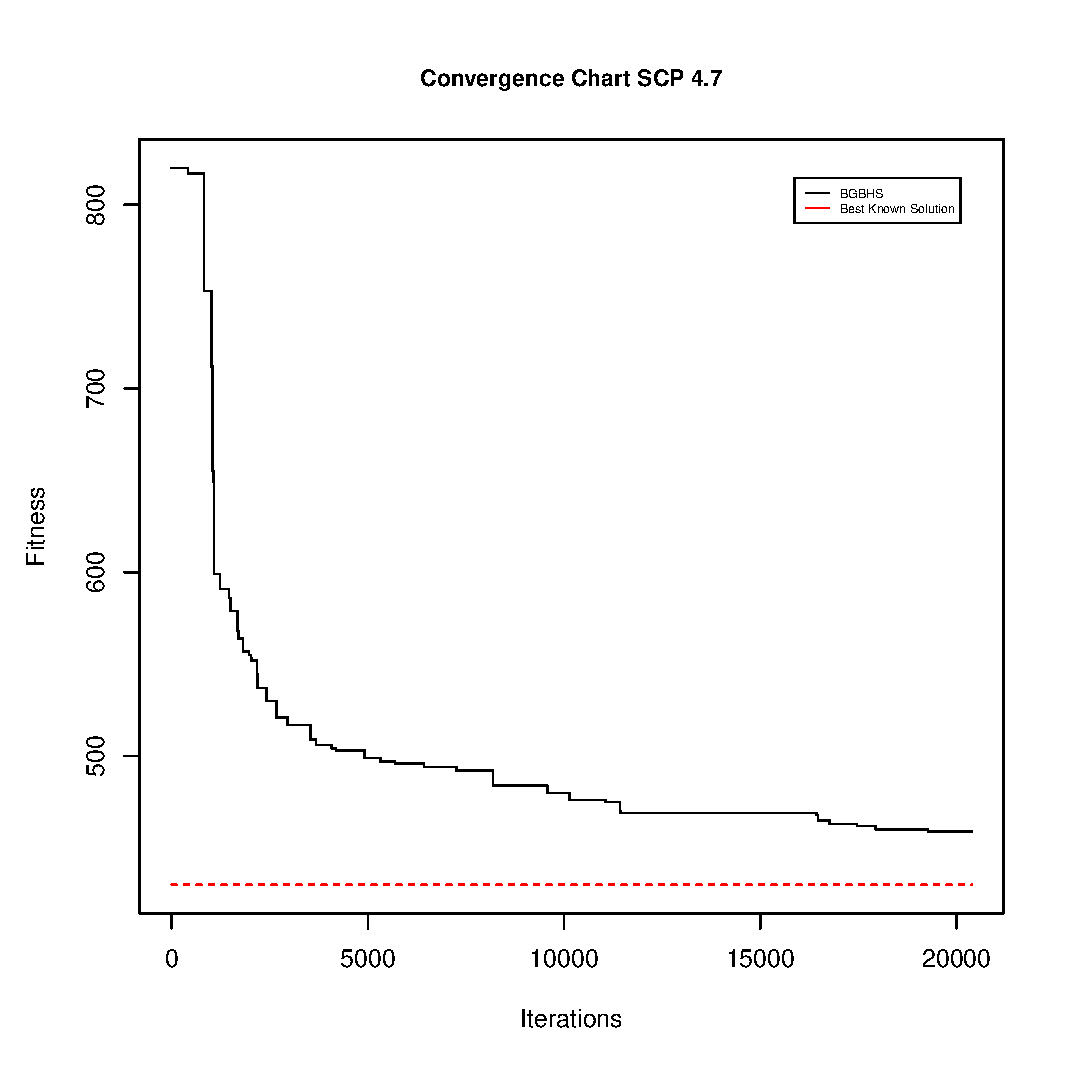
\includegraphics[scale=.45]{Resultados/scp47.eps}
\caption{Instance 4.7.}
\label{fig:Instance.4.7}
\end{figure}

%---------------------------------------------SCP48
\begin{figure}[]
\centering
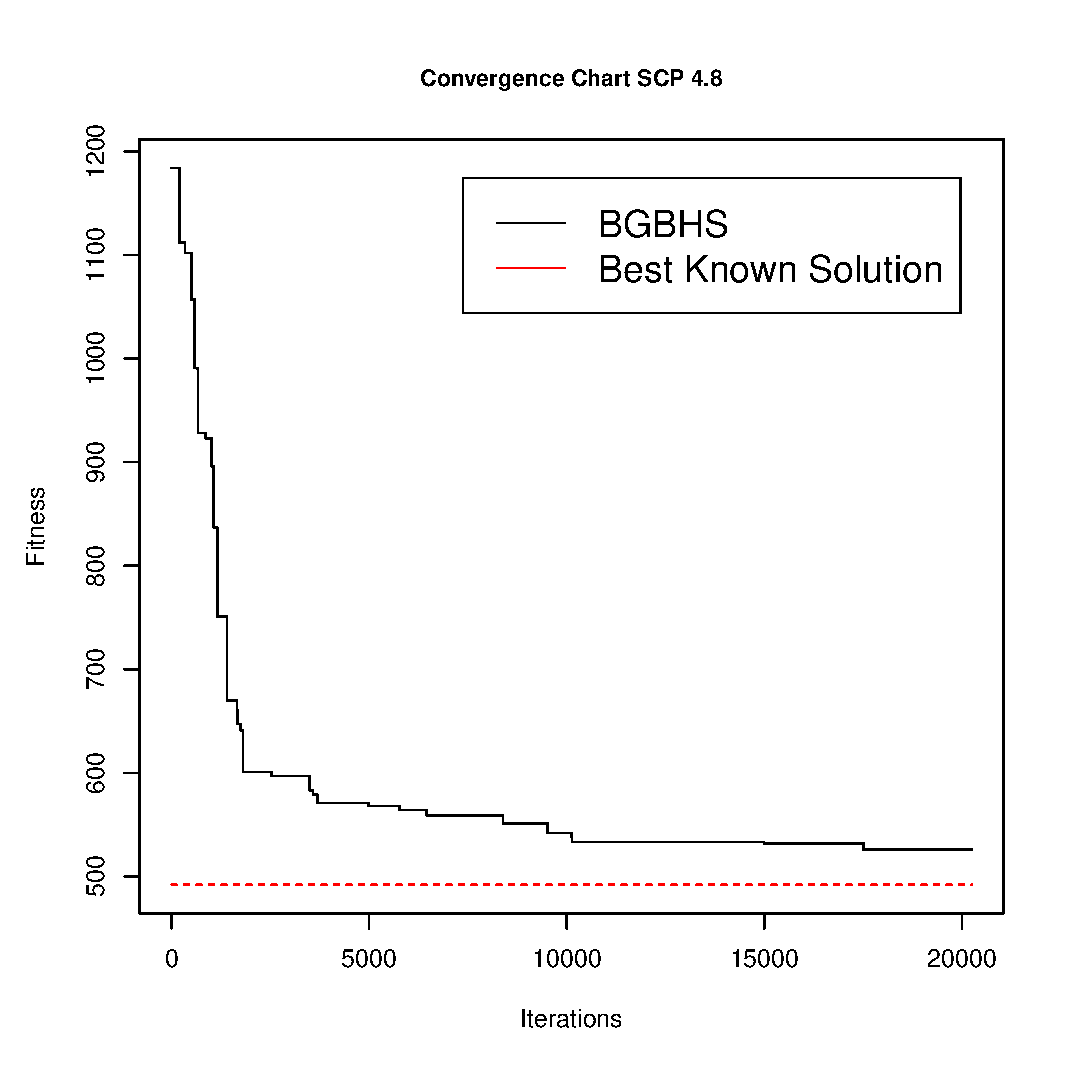
\includegraphics[scale=.45]{Resultados/scp48.eps}
\caption{Instance 4.8.}
\label{fig:Instance.4.8}
\end{figure}

%---------------------------------------------SCP49
\begin{figure}[]
\centering
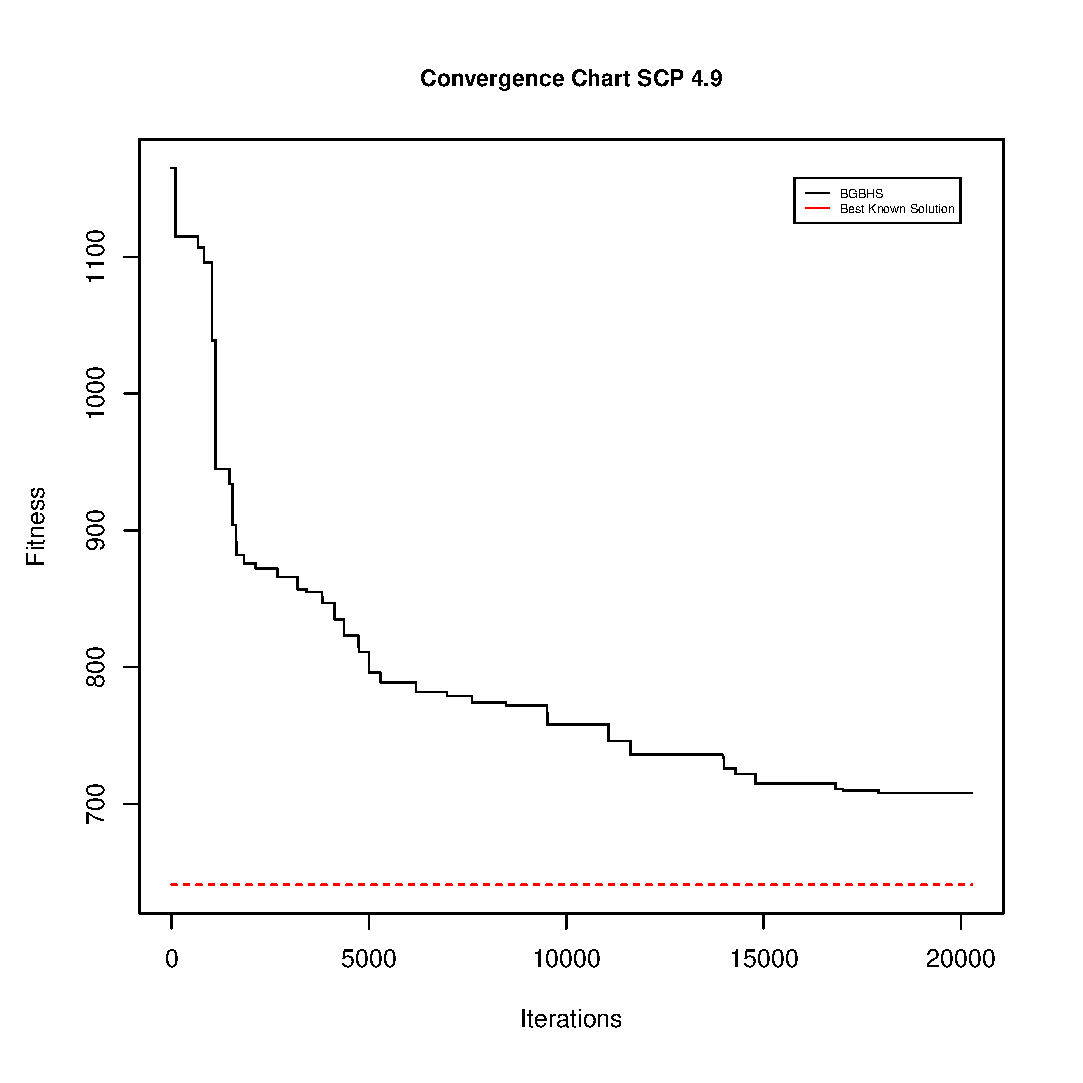
\includegraphics[scale=.45]{Resultados/scp49.eps}
\caption{Instance 4.9.}
\label{fig:Instance.4.9}
\end{figure}

%---------------------------------------------SCP410
\begin{figure}[]
\centering
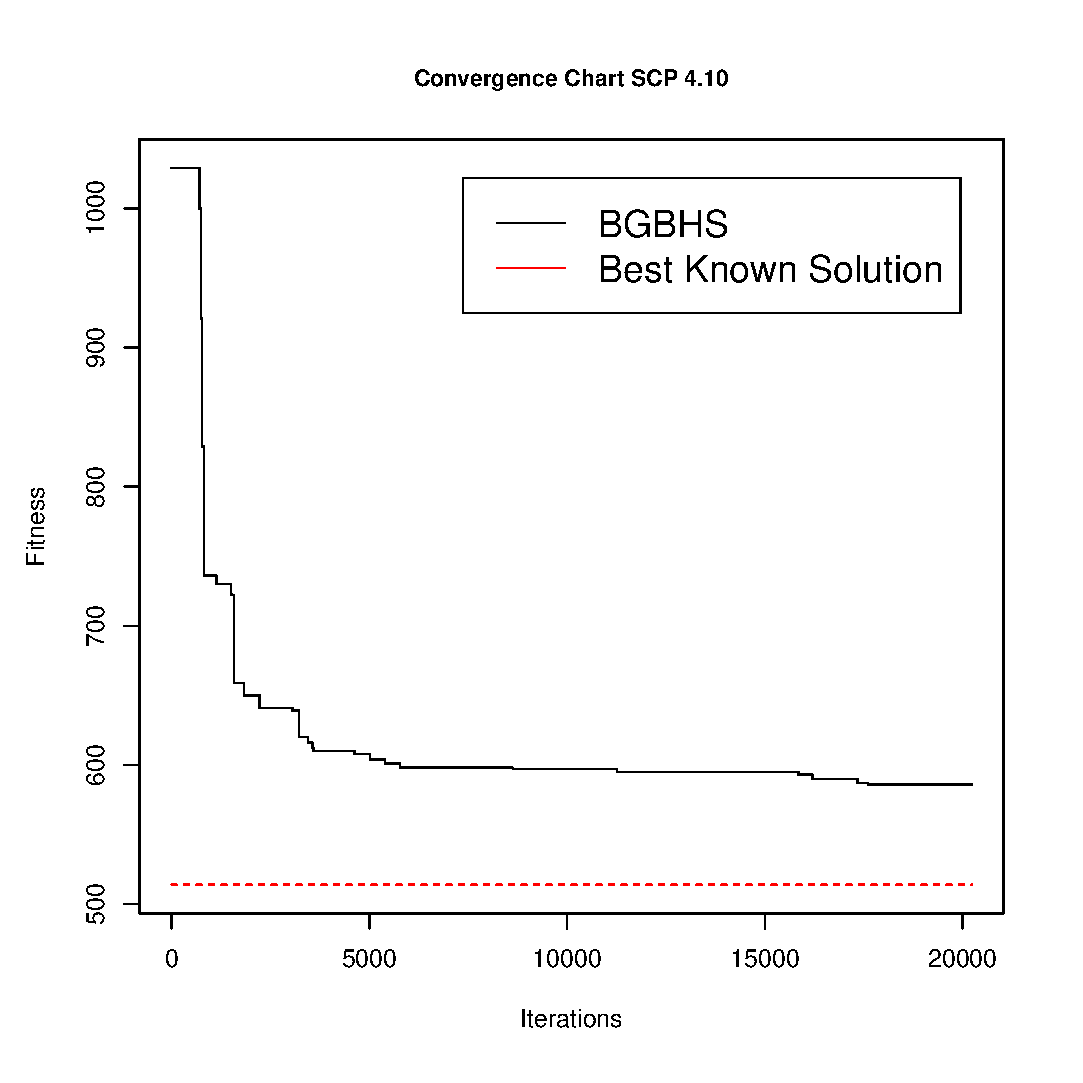
\includegraphics[scale=.45]{Resultados/scp410.eps}
\caption{Instance 4.10.}
\label{fig:Instance.4.10}
\end{figure}

%---------------------------------------------SCP51
\begin{figure}[]
\centering
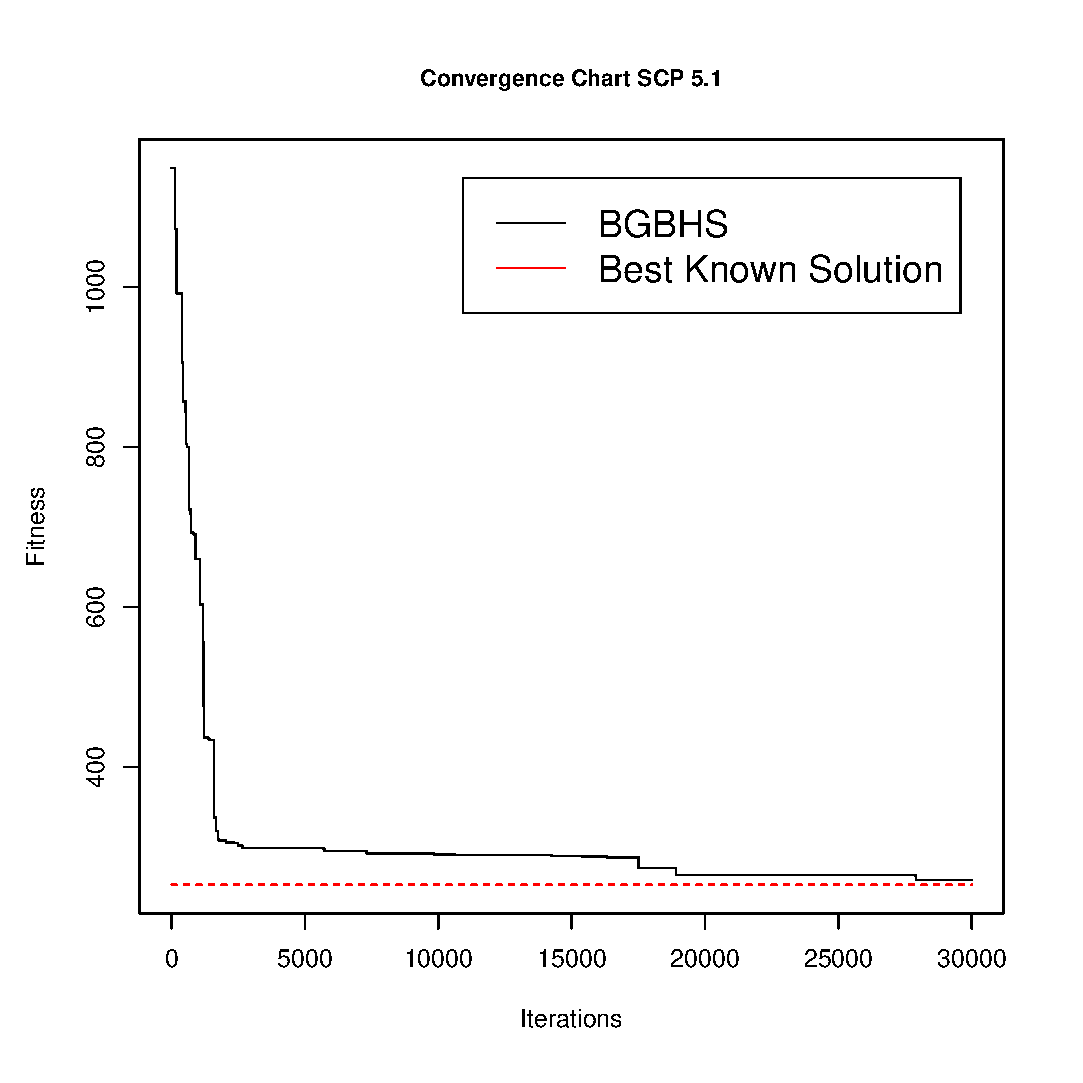
\includegraphics[scale=.45]{Resultados/scp51.eps}
\caption{Instance 5.1.}
\label{fig:Instance.5.1}
\end{figure}

%---------------------------------------------SCP52
\begin{figure}[]
\centering
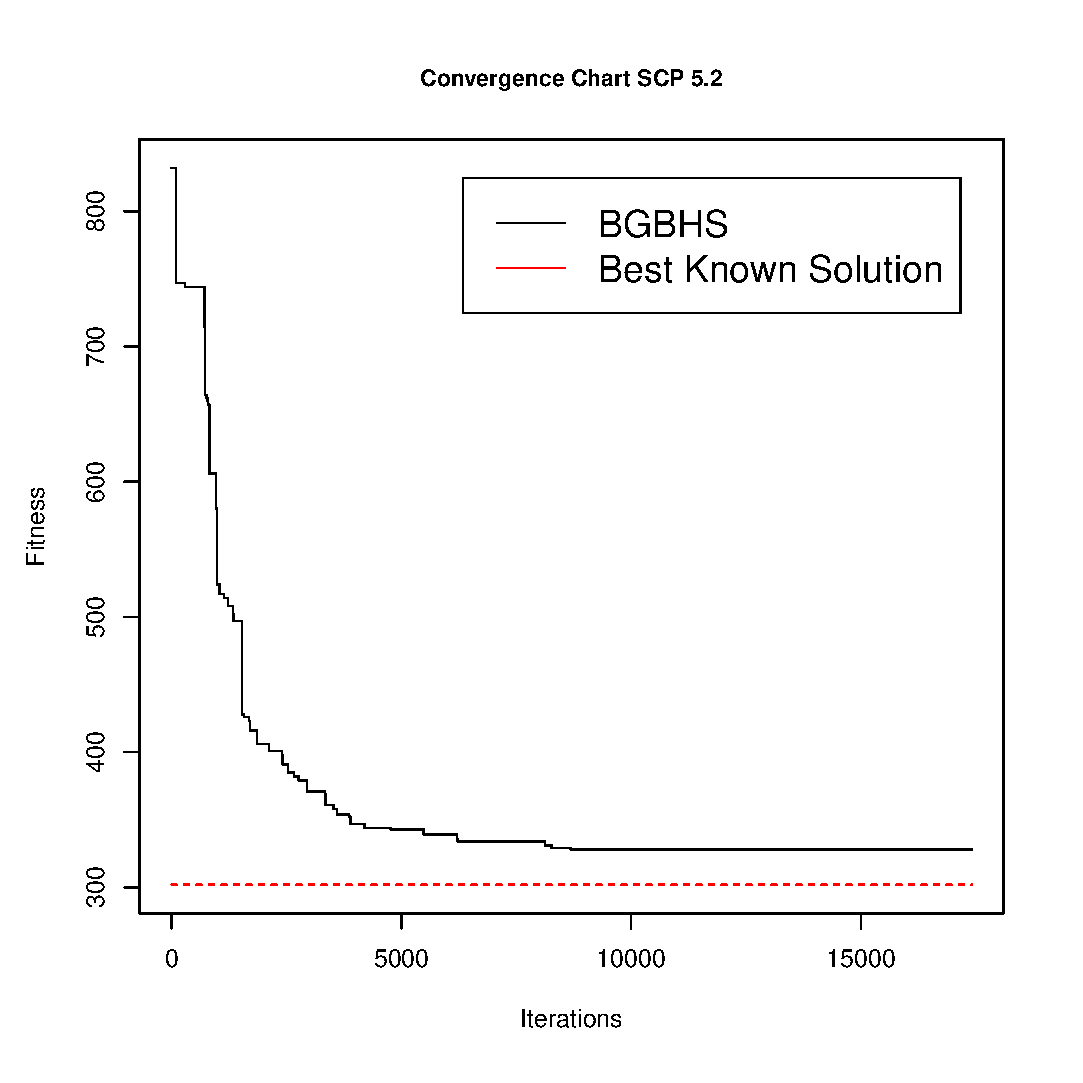
\includegraphics[scale=.45]{Resultados/scp52.eps}
\caption{Instance 5.2.}
\label{fig:Instance.5.2}
\end{figure}

%---------------------------------------------SCP53
\begin{figure}[]
\centering
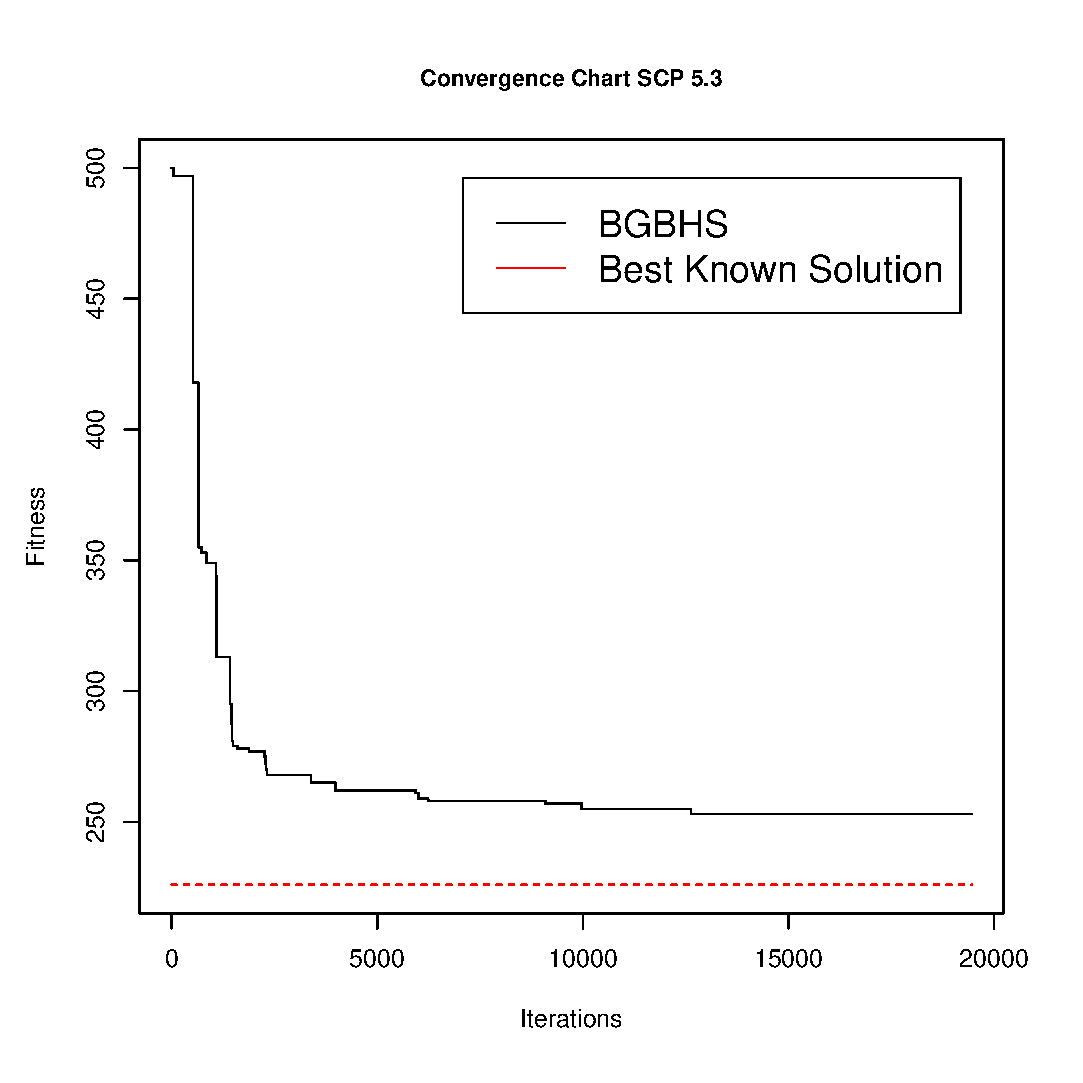
\includegraphics[scale=.45]{Resultados/scp53.eps}
\caption{Instance 5.3.}
\label{fig:Instance.5.3}
\end{figure}
%---------------------------------------------SCP54
\begin{figure}[]
\centering
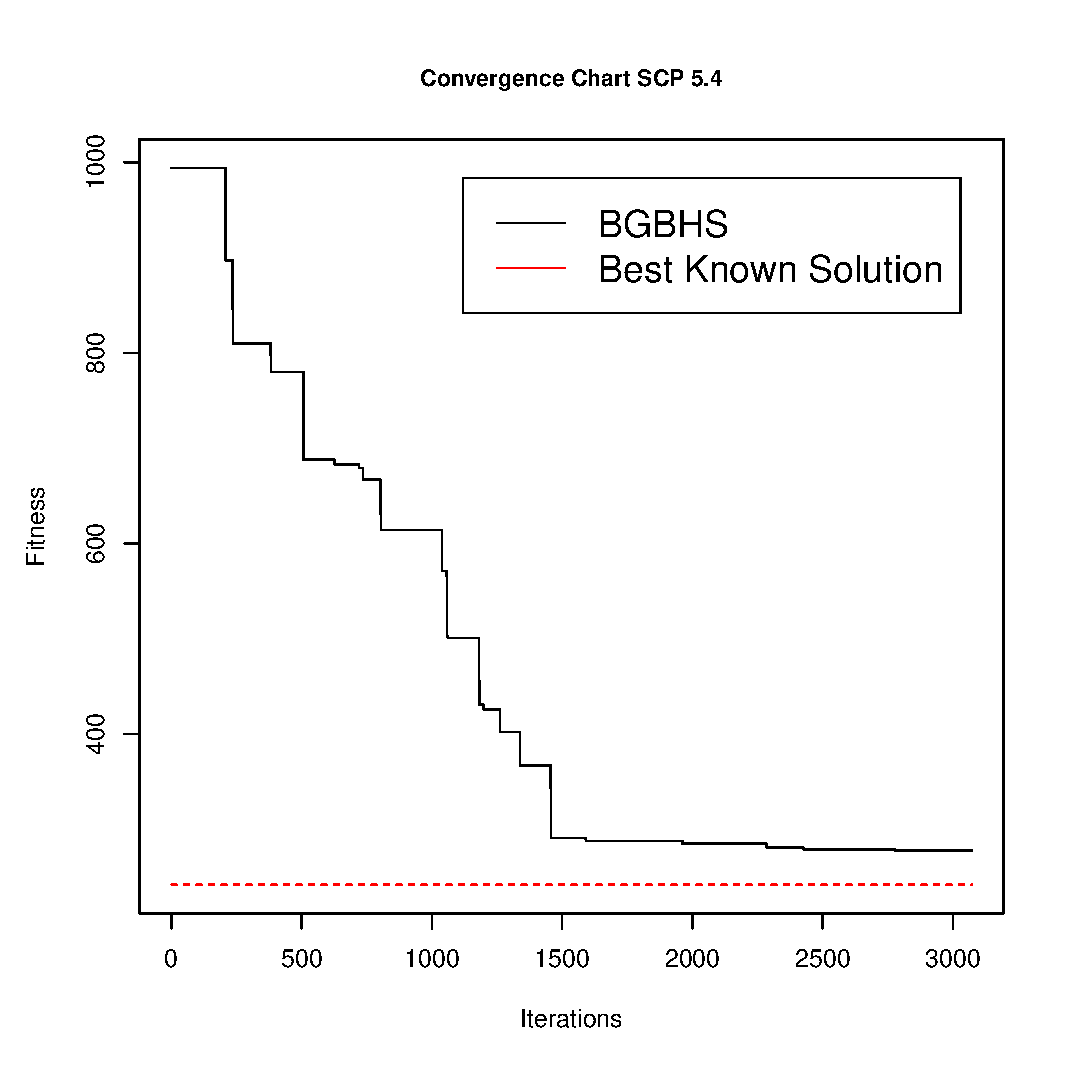
\includegraphics[scale=.45]{Resultados/scp54.eps}
\caption{Instance 5.4.}
\label{fig:Instance.5.4}
\end{figure}
%---------------------------------------------SCP55
\begin{figure}[]
\centering
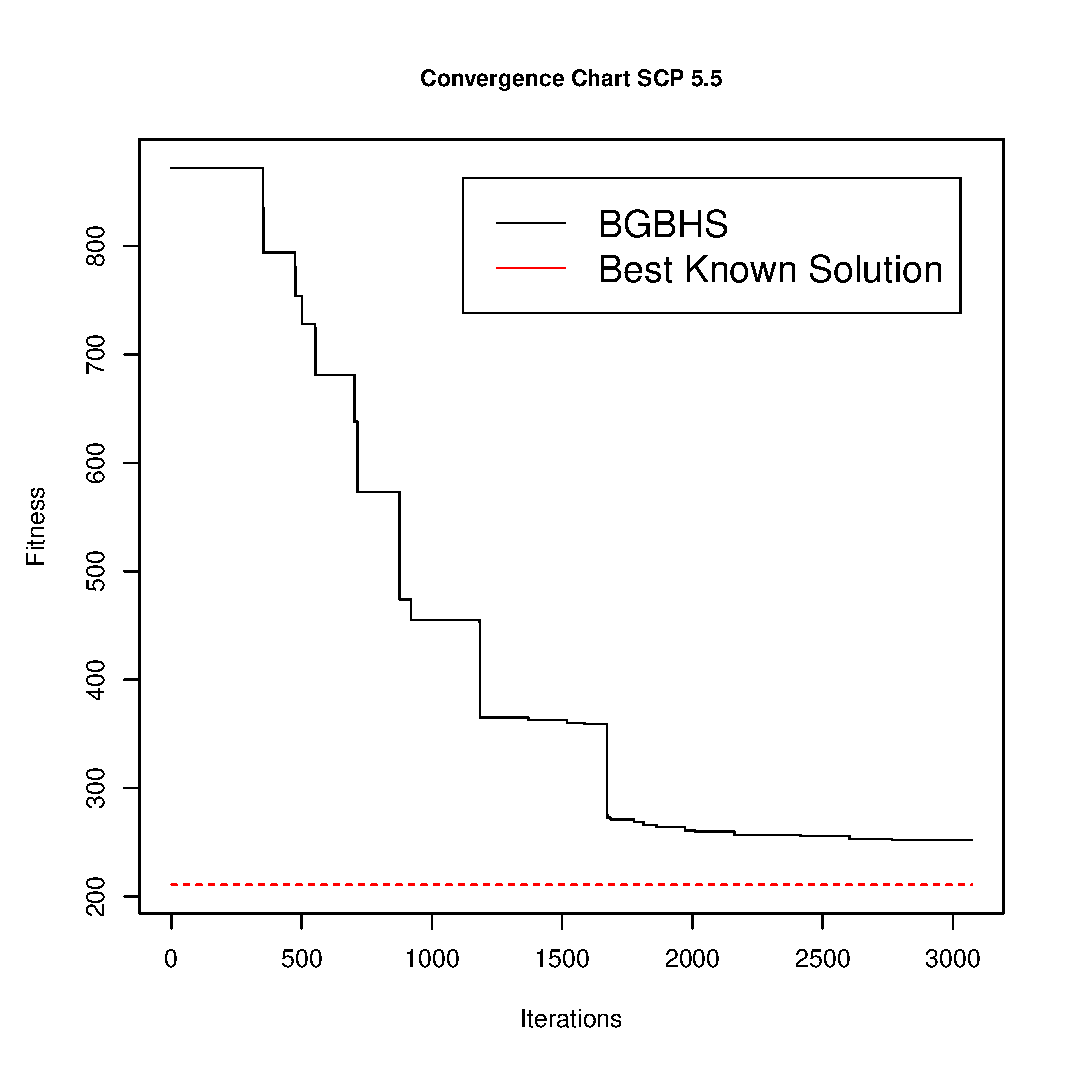
\includegraphics[scale=.45]{Resultados/scp55.eps}
\caption{Instance 5.5.}
\label{fig:Instance.5.5}
\end{figure}

%---------------------------------------------SCP56
\begin{figure}[]
\centering
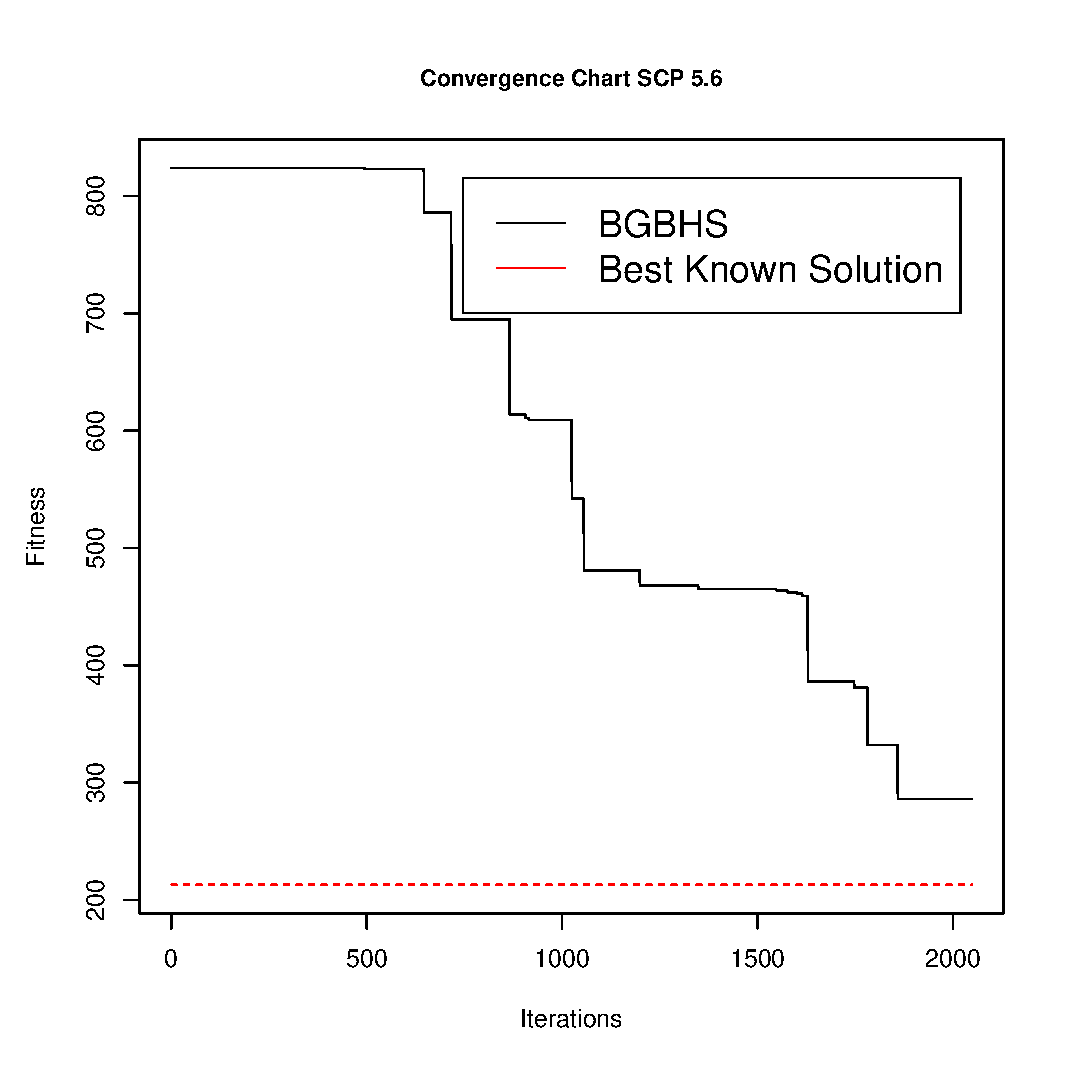
\includegraphics[scale=.45]{Resultados/scp56.eps}
\caption{Instance 5.6.}
\label{fig:Instance.5.6}
\end{figure}
%---------------------------------------------SCP57
\begin{figure}[]
\centering
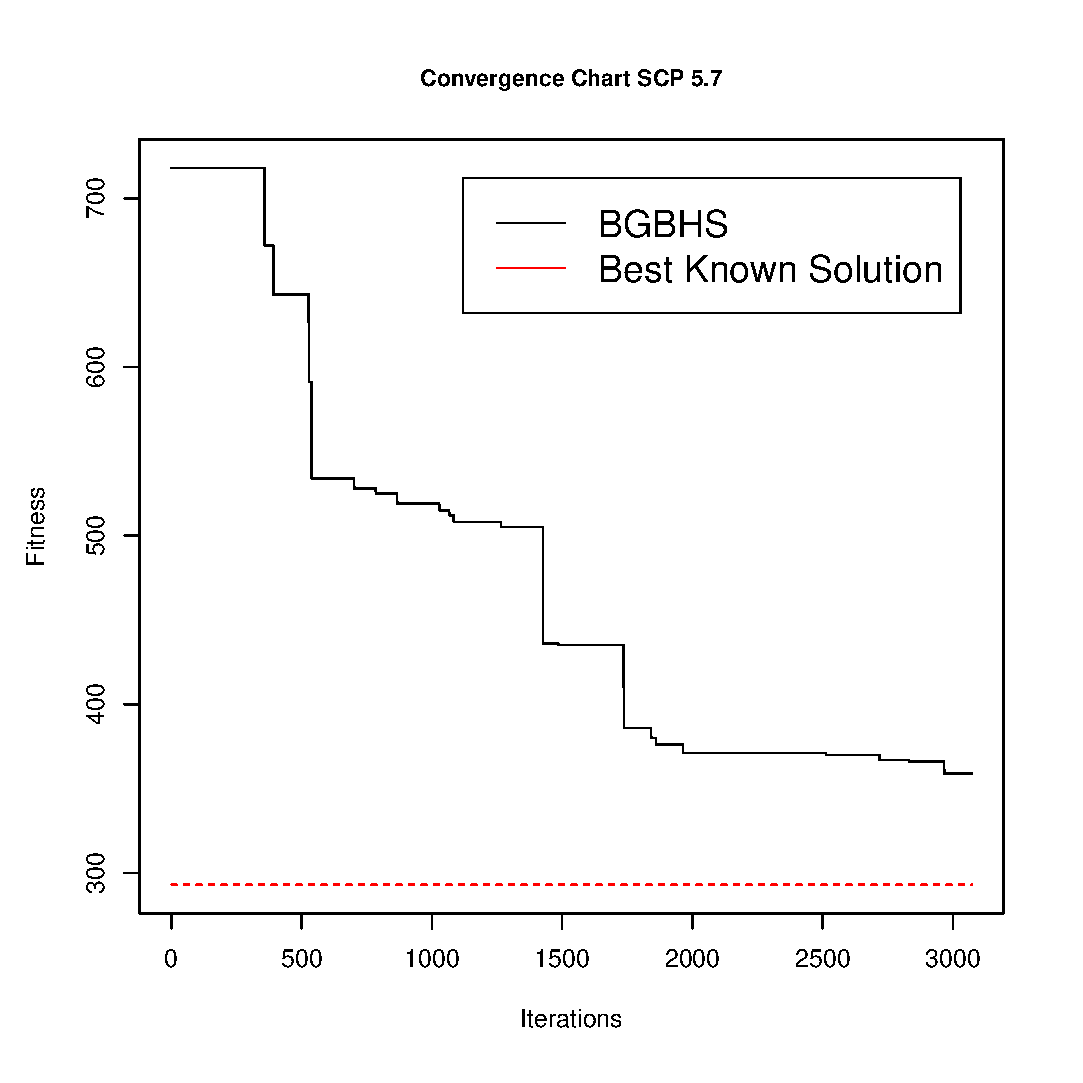
\includegraphics[scale=.45]{Resultados/scp57.eps}
\caption{Instance 5.7.}
\label{fig:Instance.5.7}
\end{figure}
%---------------------------------------------SCP58
\begin{figure}[]
\centering
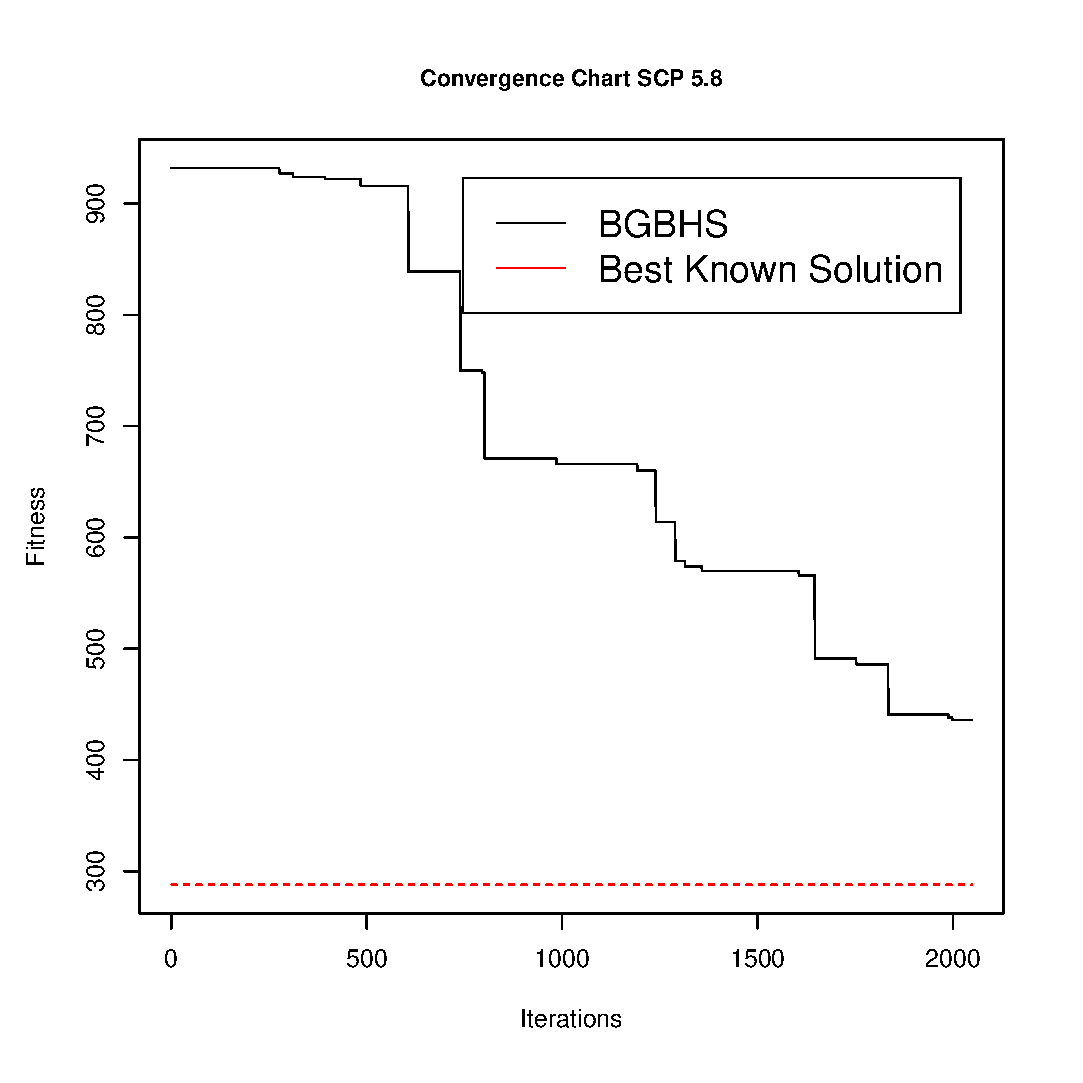
\includegraphics[scale=.45]{Resultados/scp58.eps}
\caption{Instance 5.8.}
\label{fig:Instance.5.8}
\end{figure}

%Limpieza de objetos, para liberar memoria.
\clearpage


%---------------------------------------------SCP59
\begin{figure}[]
\centering
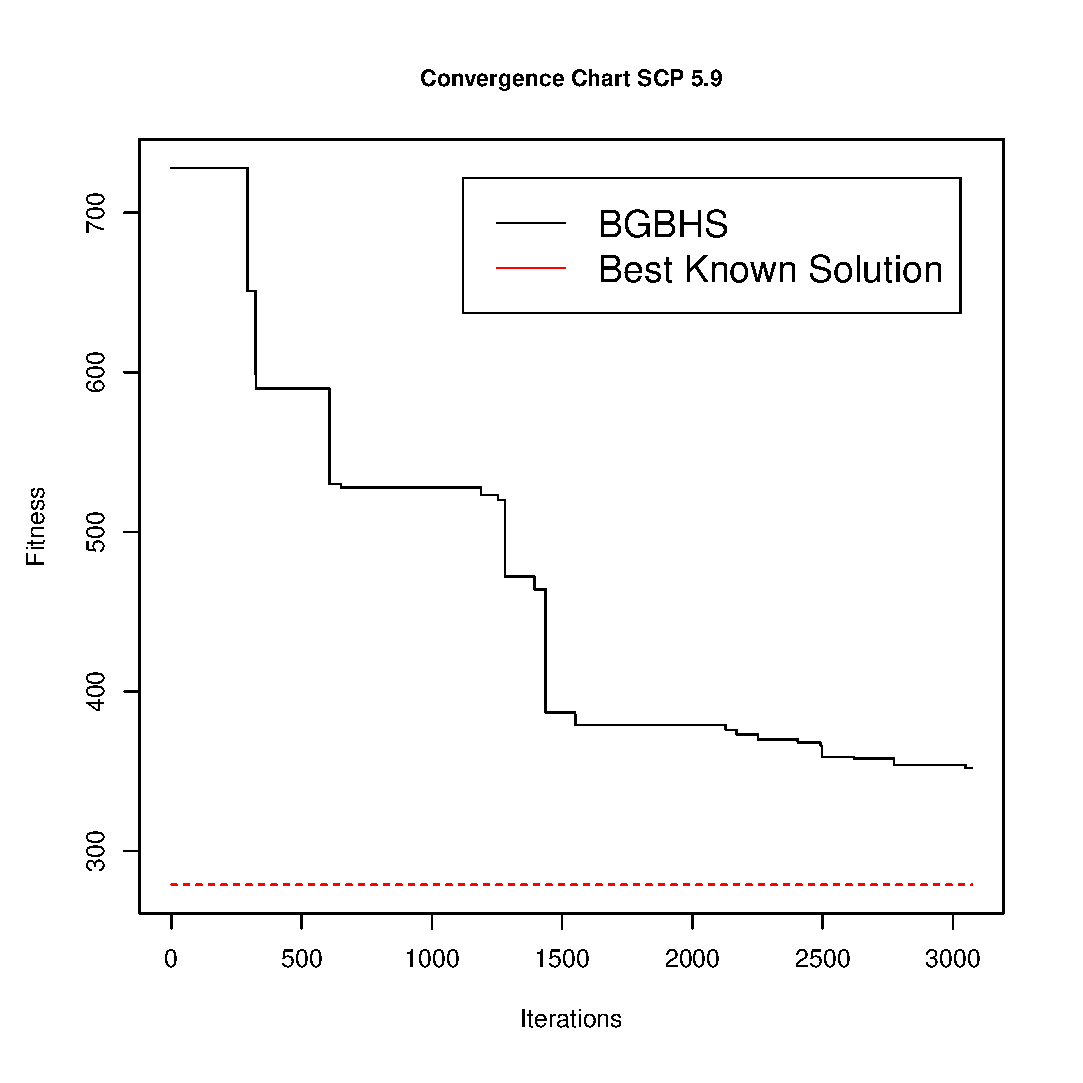
\includegraphics[scale=.45]{Resultados/scp59.eps}
\caption{Instance 5.9.}
\label{fig:Instance.5.9}
\end{figure}
%---------------------------------------------SCP510
\begin{figure}[]
\centering
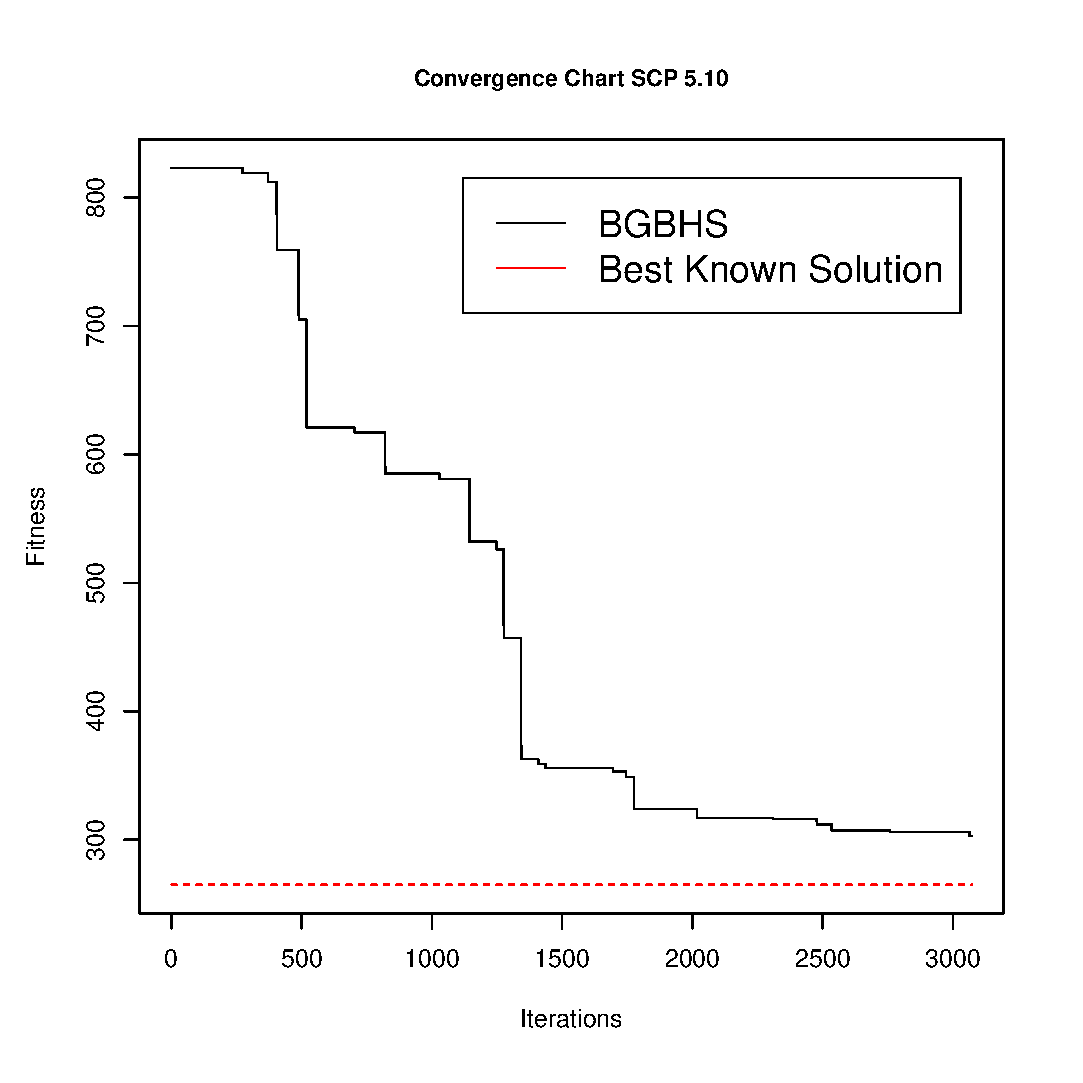
\includegraphics[scale=.45]{Resultados/scp510.eps}
\caption{Instance 5.10.}
\label{fig:Instance.5.10}
\end{figure}

%---------------------------------------------SCP61
\begin{figure}[]
\centering
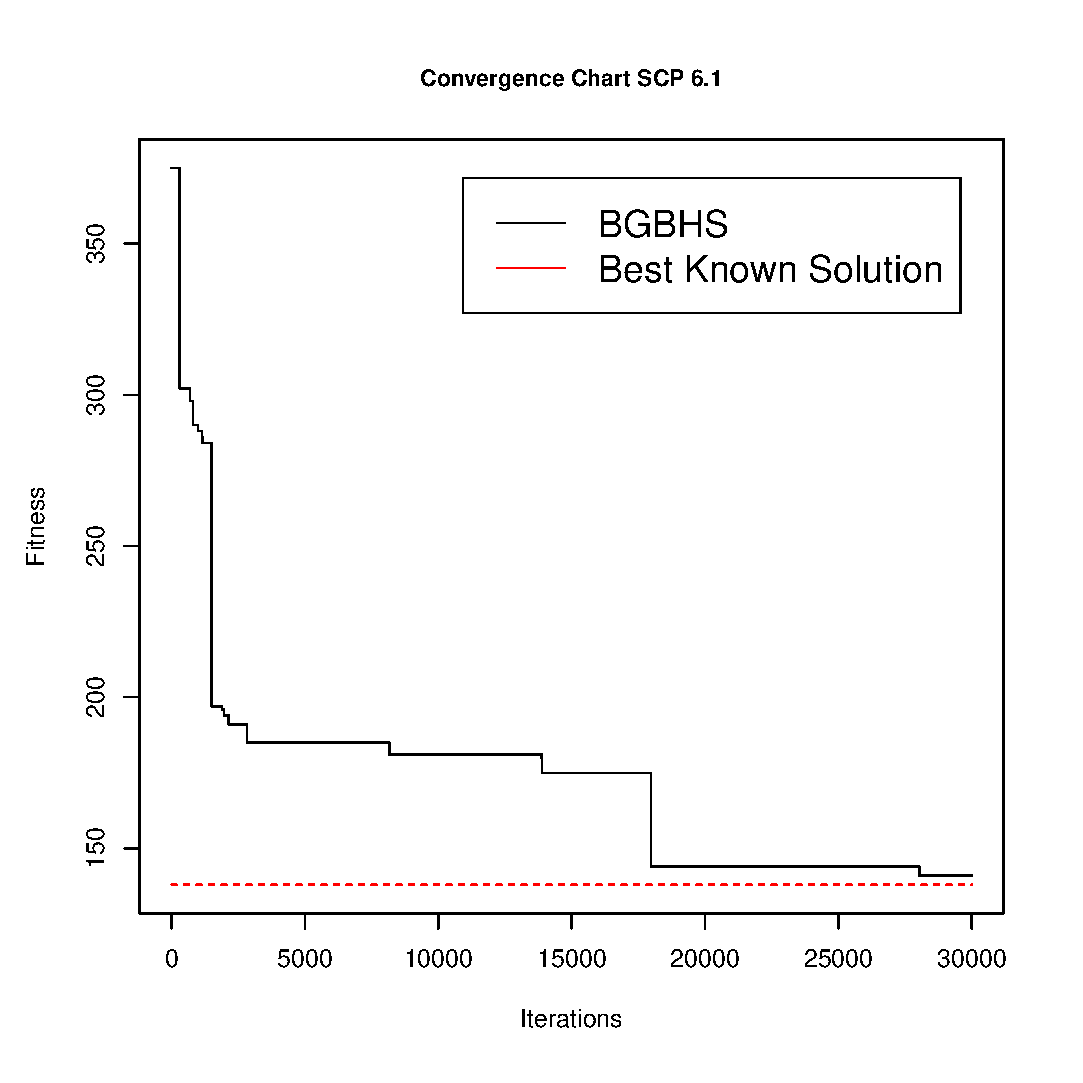
\includegraphics[scale=.45]{Resultados/scp61.eps}
\caption{Instance 6.1.}
\label{fig:Instance.6.1}
\end{figure}

%---------------------------------------------SCP62
\begin{figure}[]
\centering
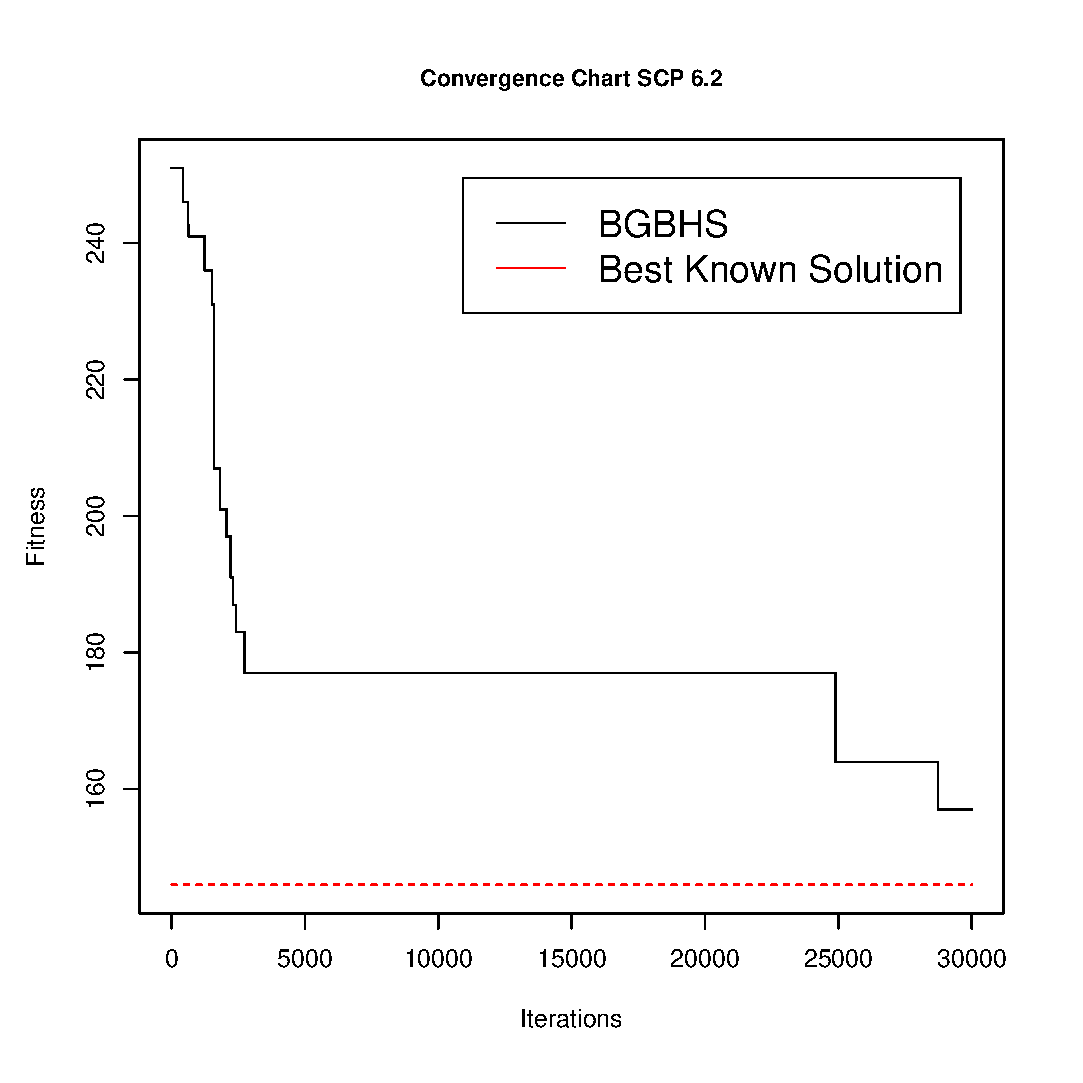
\includegraphics[scale=.45]{Resultados/scp62.eps}
\caption{Instance 6.2.}
\label{fig:Instance.6.2}
\end{figure}

%---------------------------------------------SCP63
\begin{figure}[]
\centering
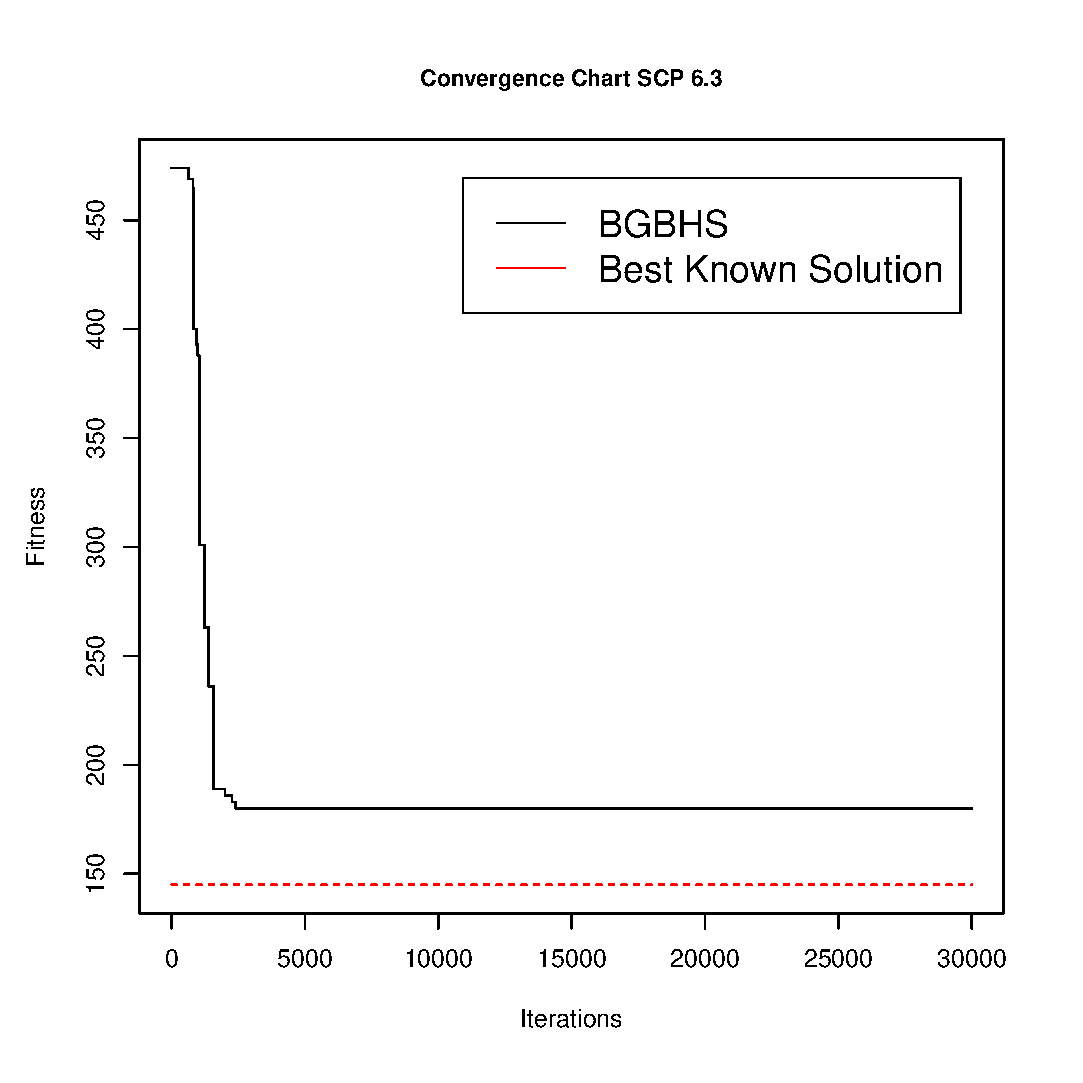
\includegraphics[scale=.45]{Resultados/scp63.eps}
\caption{Instance 6.3.}
\label{fig:Instance.6.3}
\end{figure}

%---------------------------------------------SCP64
\begin{figure}[]
\centering
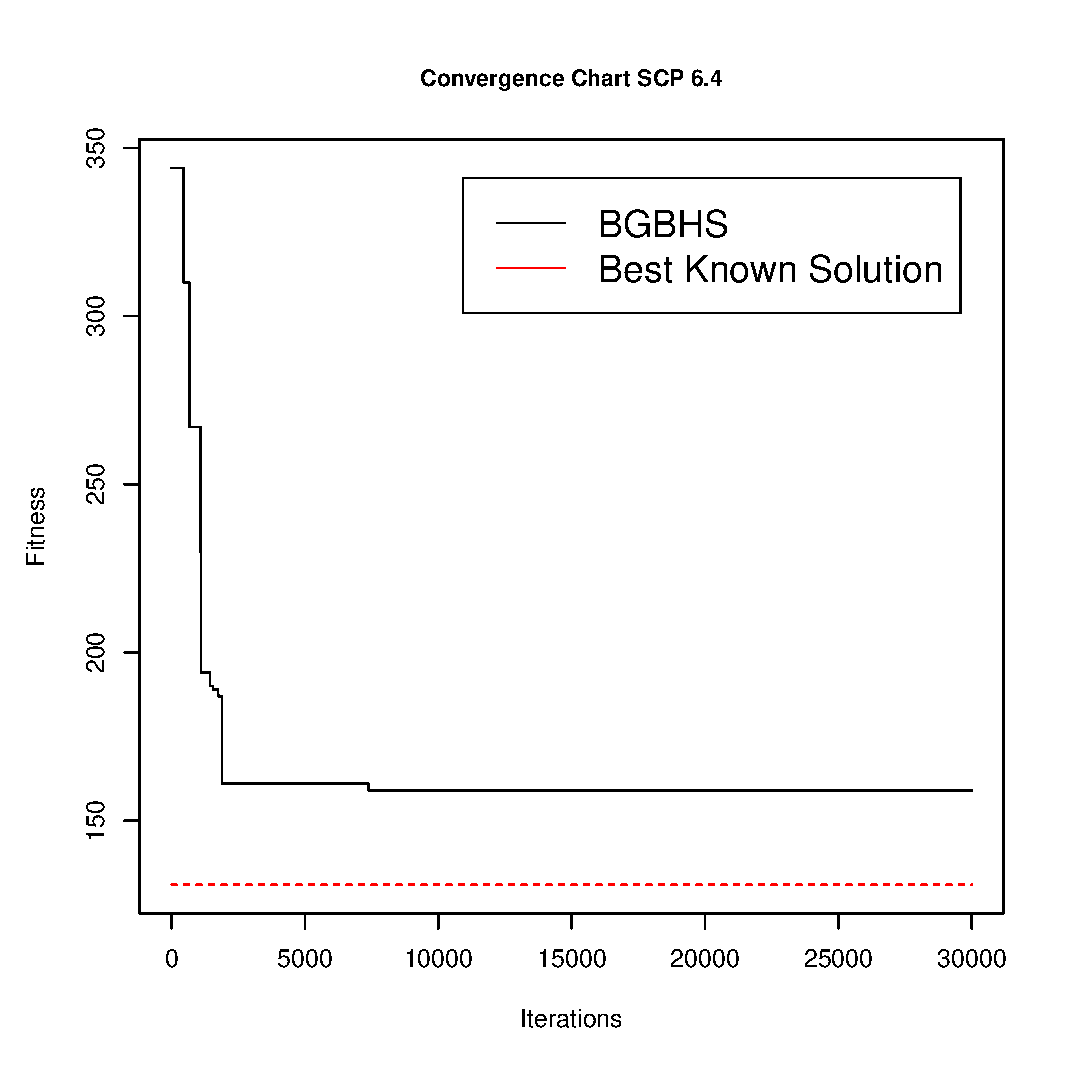
\includegraphics[scale=.45]{Resultados/scp64.eps}
\caption{Instance 6.4.}
\label{fig:Instance.6.4}
\end{figure}

%---------------------------------------------SCP65
\begin{figure}[]
\centering
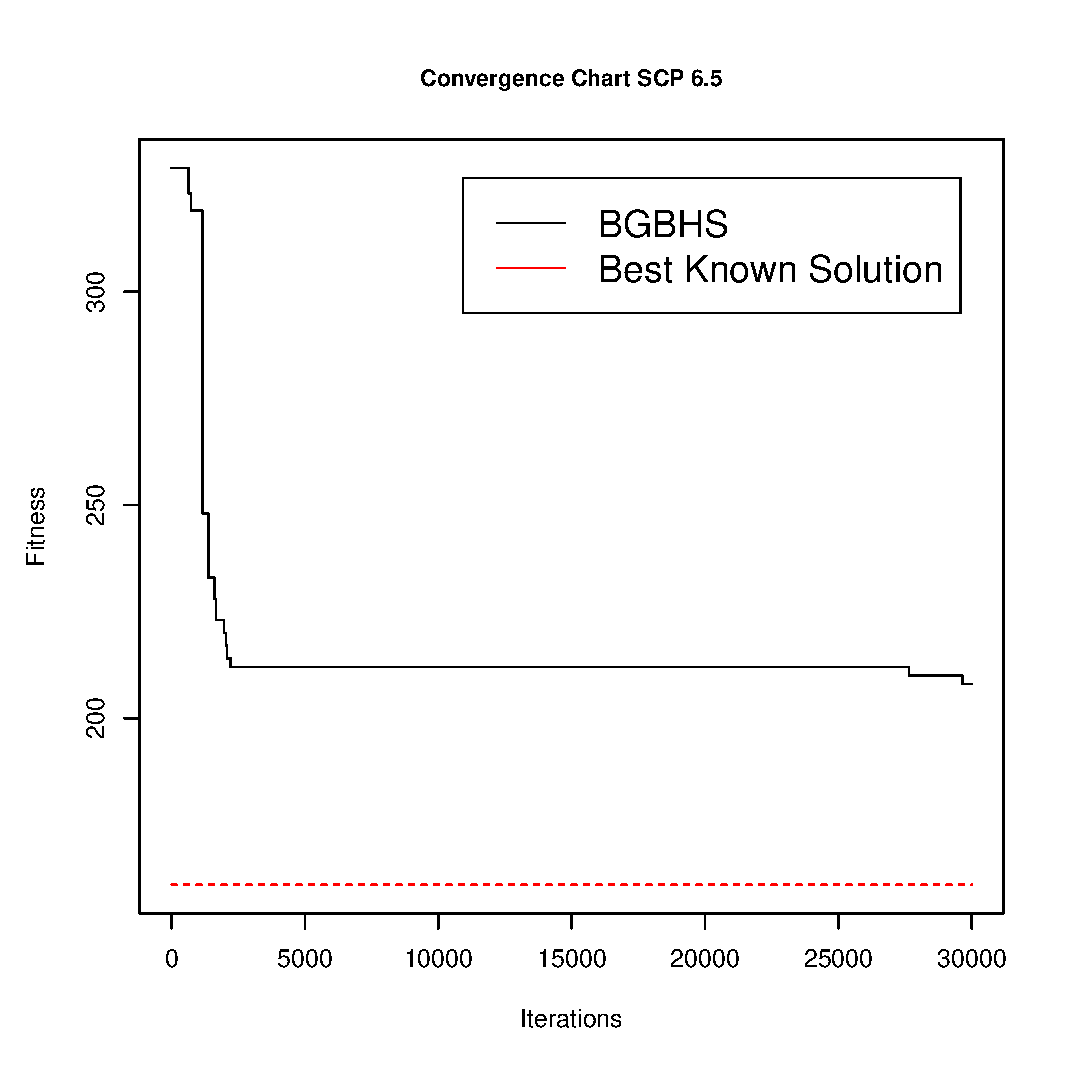
\includegraphics[scale=.45]{Resultados/scp65.eps}
\caption{Instance 6.5.}
\label{fig:Instance.6.5}
\end{figure}

%---------------------------------------------SCPA1
\begin{figure}[]
\centering
\includegraphics[scale=.45]{Resultados/scpA1.eps}
\caption{Instance A.1.}
\label{fig:Instance.A.1}
\end{figure}

%---------------------------------------------SCPA2
\begin{figure}[]
\centering
\includegraphics[scale=.45]{Resultados/scpA2.eps}
\caption{Instance A.2.}
\label{fig:Instance.A.2}
\end{figure}

%---------------------------------------------SCPA3
\begin{figure}[]
\centering
\includegraphics[scale=.45]{Resultados/scpA3.eps}
\caption{Instance A.3.}
\label{fig:Instance.A.3}
\end{figure}

%---------------------------------------------SCPA4
\begin{figure}[]
\centering
\includegraphics[scale=.45]{Resultados/scpA4.eps}
\caption{Instance A.4.}
\label{fig:Instance.A.4}
\end{figure}

%---------------------------------------------SCPA5
\begin{figure}[]
\centering
\includegraphics[scale=.45]{Resultados/scpA5.eps}
\caption{Instance A.5.}
\label{fig:Instance.A.5}
\end{figure}

%---------------------------------------------SCPB1
\begin{figure}[]
\centering
\includegraphics[scale=.45]{Resultados/scpB1.eps}
\caption{Instance B.1.}
\label{fig:Instance.B.1}
\end{figure}

%---------------------------------------------SCPB2
\begin{figure}[]
\centering
\includegraphics[scale=.45]{Resultados/scpB2.eps}
\caption{Instance B.2.}
\label{fig:Instance.B.2}
\end{figure}

%Limpieza de objetos, para liberar memoria.
\clearpage

%---------------------------------------------SCPB3
\begin{figure}[]
\centering
\includegraphics[scale=.45]{Resultados/scpB3.eps}
\caption{Instance B.3.}
\label{fig:Instance.B.3}
\end{figure}

%---------------------------------------------SCPB4
\begin{figure}[]
\centering
\includegraphics[scale=.45]{Resultados/scpB4.eps}
\caption{Instance B.4.}
\label{fig:Instance.B.4}
\end{figure}

%---------------------------------------------SCPB5
\begin{figure}[]
\centering
\includegraphics[scale=.45]{Resultados/scpB5.eps}
\caption{Instance B.5.}
\label{fig:Instance.B.5}
\end{figure}

%---------------------------------------------SCPC1
\begin{figure}[]
\centering
\includegraphics[scale=.45]{Resultados/scpC1.eps}
\caption{Instance C.1.}
\label{fig:Instance.C.1}
\end{figure}

%---------------------------------------------SCPC2
\begin{figure}[]
\centering
\includegraphics[scale=.45]{Resultados/scpC2.eps}
\caption{Instance C.2.}
\label{fig:Instance.C.2}
\end{figure}

%---------------------------------------------SCPC3
\begin{figure}[]
\centering
\includegraphics[scale=.45]{Resultados/scpC3.eps}
\caption{Instance C.3.}
\label{fig:Instance.C.3}
\end{figure}

%---------------------------------------------SCPC4
\begin{figure}[]
\centering
\includegraphics[scale=.45]{Resultados/scpC4.eps}
\caption{Instance C.4.}
\label{fig:Instance.C.4}
\end{figure}

%---------------------------------------------SCPC5
\begin{figure}[]
\centering
\includegraphics[scale=.45]{Resultados/scpC5.eps}
\caption{Instance C.5.}
\label{fig:Instance.C.5}
\end{figure}

%---------------------------------------------SCPD1
\begin{figure}[]
\centering
\includegraphics[scale=.45]{Resultados/scpD1.eps}
\caption{Instance D.1.}
\label{fig:Instance.D.1}
\end{figure}

%---------------------------------------------SCPD2
\begin{figure}[]
\centering
\includegraphics[scale=.45]{Resultados/scpD2.eps}
\caption{Instance D.2.}
\label{fig:Instance.D.2}
\end{figure}

%---------------------------------------------SCPD3
\begin{figure}[]
\centering
\includegraphics[scale=.45]{Resultados/scpD3.eps}
\caption{Instance D.3.}
\label{fig:Instance.D.3}
\end{figure}

%---------------------------------------------SCPD4
\begin{figure}[]
\centering
\includegraphics[scale=.45]{Resultados/scpD4.eps}
\caption{Instance D.4.}
\label{fig:Instance.D.4}
\end{figure}

%---------------------------------------------SCPD5
\begin{figure}[]
\centering
\includegraphics[scale=.45]{Resultados/scpD5.eps}
\caption{Instance D.5.}
\label{fig:Instance.D.5}
\end{figure}
  \newpage
  
  \section{Analysis of results}\label{sec:Analisys}
  In this chapter we will perform an analysis of the results obtained in the multiple experiments. The analysis will allow us to obtain information regarding the original algorithm and compare it with the improved algorithm. In the same way we will compare the results with those obtained by other metaheuristics.

\subsection{Comparison of results}
In order to be able to present a correct analysis, a summary table (Table~\ref{tblRpdComparison}) is made comparing the RPDs averages of each value of the groups of instances. These are presented in such a way that allows us to objectively observe the behavior of metaheuristics in the face of a given problem and a set of known data, as already mentioned in the beginning of this work.

In the summary table we can see that each record of the first column identifies the group of instances that was observed and measured. Each record in the second column refers to an average RPD for the BGBHS metaheuristic developed without any improvement. The following column shows the RPD averages for the BGBHS metaheuristic with the improvement associated with the variation of the $ p $ parameter in the Bernoulli trial. The following column refers to the averages of RPD per instance of the BH S-Shape algorithm and finally the BH Improved column refers to the RPD averages of this metaheuristic. Finally the last row, generalizes a total of all RPD for each algorithm tested, in order to make a single final analysis.

\begin{table}[H]
\centering
\begin{tabular}{|c|c|c|c|c|}
\hline
\multicolumn{1}{|l|}{\textbf{\begin{tabular}[c]{@{}l@{}}Instance\\ group\end{tabular}}} & \multicolumn{1}{l|}{\textbf{\begin{tabular}[c]{@{}l@{}}BGBHS \\ average RPD\end{tabular}}} & \multicolumn{1}{l|}{\textbf{\begin{tabular}[c]{@{}l@{}}BGBHS \\ Improved\\ average RPD\end{tabular}}} & \multicolumn{1}{l|}{\textbf{\begin{tabular}[c]{@{}l@{}}Black Hole\\ S-Shape\\ average RPD\end{tabular}}} & \multicolumn{1}{l|}{\textbf{\begin{tabular}[c]{@{}l@{}}Black Hole\\ Improved\\ average RPD\end{tabular}}} \\ \hline
4                                                                                       & 8.55                                                                                       & 1.12                                                                                                  & 7.66                                                                                                     & 2.28                                                                                                      \\ \hline
5                                                                                       & 20.71                                                                                      & 2.42                                                                                                  & 12.41                                                                                                    & 4.83                                                                                                      \\ \hline
6                                                                                       & 16.88                                                                                      & 1.53                                                                                                  & 13.80                                                                                                    & 7.74                                                                                                      \\ \hline
A                                                                                       & 15.61                                                                                      & 4.63                                                                                                  & 18.94                                                                                                    & 14.96                                                                                                     \\ \hline
B                                                                                       & 74.28                                                                                      & 6.14                                                                                                  & 24.89                                                                                                    & 18.79                                                                                                     \\ \hline
C                                                                                       & 24.25                                                                                      & 5.35                                                                                                  & 12.78                                                                                                    & 11.07                                                                                                     \\ \hline
D                                                                                       & 65.87                                                                                      & 11.42                                                                                                 & 22.78                                                                                                    & 14.20                                                                                                     \\ \hline
\multicolumn{1}{|l|}{\textbf{TOTAL}}                                                    & \textbf{32.31}                                                                             & \textbf{4.66}                                                                                         & \textbf{16.18}                                                                                           & \textbf{10.55}                                                                                            \\ \hline
\end{tabular}
\caption{RPD comparison}
\label{tblRpdComparison}
\end{table}


Regarding the group of instances 4, we can see that the worst result (8.55) in averages of RPD was for BGBHS in its version without improvements, whereas the best result (1.12) was for BGBHS with improvements. The best solution was followed closely by BH with improvements (2.28).\\

In the group of instances 5, a result very similar to 4 is produced. Where the worst RPD average result (20.71) was for BGBHS and the best (2.42) was for improved BGBHS, equally BH improved (4.83) closely follows the best average.\\

In the grouping of instances 6, the same pattern is followed as with the two cases previously reviewed, where the best RPD average (1.53) is for improved BGBHS and the worst result (16.88) is for traditional BGBHS. In this set of instances, there is a gap between improved BGBHS and BH improved by almost 6 points, although the same order is maintained when ranking from best to worst.\\

In the group of instances A, the tendency is broken, since the worst result in averages of RPD is for BH S-Shape (18.94) and the average between traditional BGBHS and improved BH is quite close with 0.61 difference. The best result continues to be for BGBHS with improvements (4.63).\\

For the group of instances B, we obtained the worst result in average RPD (74.28) for the metaheuristic BGBHS, even worse was the worst result of all sets of instances. Consistently the best result in averages of RPD was for BGBHS in its improved version. This time the gap between the best version of BGBHS and BH, distanced in 12.65, giving the advantage to BGBHS.\\

In the group of instances of C, we can see that the worst result in RPD averages obtained (24.25) was for BGBHS in its traditional version, while the best result in RPD averages (5.35) was for BGBHS in its improved version. They maintain a distance of 5.72 between the best average of BGBHS and the best of BH.\\

Finally in the group of instances D, the worst result in average RPD (65.87) was obtained by the metaheuristic BGBHS in its traditional version. The best result obtained in averages of RPD was obtained by BGBHS in its improved version. In this opportunity the distance between the best version of BGBHS and BH, decreased with respect to the group of previous instances, arriving at 2.78.\\

When we globally analyze the averages in RPD of all the results of each instance, Total row of the table \ ref {tblRpdComparison}, we can see that the trend analyzed in each group of instances is maintained.
The worst overall result is 32.31, which corresponds to the metaheuristic BGBHS in its classic version. On the other hand the best result on average RPD 4.66 corresponds to BGBHS in its improved version. When comparing the best overall RPD of BGBHS against BH, there is a difference of 6.49 in favor of Harmony Search.\\

Our results show that the improved version of BGBHS consistently beats BH in the two versions evaluated. On the other hand, the version of BGBHS in its classic version is beaten in all groups of instances by improved BH and in almost all BH S-Shape units except for instance group 6. The analyzes can be appreciated in the Figure~\ref{fig:RPDAverage}.\\

\begin{figure}[H]
\centering
\includegraphics[scale=.55]{Analisys/comparisionGraph.eps}
\caption{RPD average in each instance}
\label{fig:RPDAverage}
\end{figure}

Graphical representation of convergence can be seen in appendix section \ref{sec:Anexo}. Within this section you will be able to see comparative graphs for BGBHS and BGBHS Improved, in such a way that it is evident the improvement that occurs in exploration (Figures~\ref{fig:Instance.4.1}, \ref{fig:Instance.5.1} and \ref{fig:Instance.6.1}).


  \newpage
  
    \section{Conclusion}\label{sec:Conclusi�n}
  In this chapter, a general conclusion of the work will be addressed, starting from the basis of the exhaustive detail seen in chapter \ref{sec:Analisys}.
We will then move on to a view of the overall results compared to other metaheuristics. Finally, we will make an approach that lay the foundation for future work.

\subsection{Global analysis}
This work began with the need to obtain a thorough knowledge of metaheuristics, with the ultimate aim of getting into the world of information security and to be able to apply this method in it future works. In order to achieve this goal the first thing was to know in depth how a metaheuristic worked, for it was studied in detail the behavior of several algorithms
To find one that met certain characteristics that made it interesting to study. In this case, Harmony Search was selected.\\

Once the algorithm or metaheuristic was selected the next step was to confront the decision to choose a type problem, to which to apply the metaheuristic and to look for possible solutions. According to what was reviewed in different publications \cite{DBLP:journals/eswa/Lanza-Gutierrez17, DBLP:conf/csoc/CrawfordSAO16,DBLP:conf/csoc/CrawfordSBO16}, SCP was chosen because it had broad applications and was easy to implement.\\

After having selected Harmony Search and SCP, it is necessary to review the behavior against other metaheuristics, for which it is necessary to use a set of known data, for which we use the library of J.E.Beasley.\\

After specifying the above, we evaluated the behavior of the selected metaheuristics BGBHS, compared to others with similar characteristics. As you can see in the analysis and results section. The selected metaheuristic presents poor performance in relation to Black Hole S-Shape and Improved Black Hole, according to RPD measurements.\\

Considering the comparative results of the RPDs obtained, the need to improve BGBHS was presented, for which a novel method is proposed that aims to achieve a wider variation in the initial population of solutions, thus obtaining a better convergence, but mainly a better exploration since the solutions depart being feasible but not so close to optimum then vary until they are feasible and close to the optimum.\\

The results improved ostensibly, when comparing BGBHS optimized, with BH S-Shape and BH Enhanced. If we look at the curves proposed in Comparison graph of RPD (Fig.~\ref{fig:RPDAverage}), we can see that the curve associated to optimized BGBHS has a lower elevation than the averages of RPD per instances. This clearly demonstrates through many experiments that the metaheuristic has a stable and effectively better behavior than BH in the two versions evaluated. In spite of all the experiments performed and having a stable behavior and better than some metaheuristics, it is not possible to reach the global optimum.\\

The path traveled shows that a minimum knowledge has been achieved, this allows to make use of a metaheuristic in any problem and in any domain. All the main and specific objectives were met.\\

As future work, it is proposed the application of different metaheuristics in the field of IT security, trying to improve existing applications, looking for viruses and other threats \cite{Edge_aretrovirus, Mehdi:2009:IIM:1569901.1570109, Noreen:2009:EM:1569901.1570111, Shafiq:2009:AER:1570256.1570370, NajwadiYusoff00000060, DBLP:conf/iccci/DemertzisI15}.















  \newpage

  \section{Appendix}\label{sec:Anexo}
  %---------------------------------------------SCP41 (Con y Sin B)
\begin{figure}[htp] 
    \centering
    \subfloat[]{%
        \includegraphics[width=0.45\textwidth]{Resultados/scp41_sb.eps}%
        \label{fig:b}%
        }%    
    \hfill%
    \subfloat[]{%
        \includegraphics[width=0.45\textwidth]{Resultados/scp41.eps}%
        \label{fig:a}%
        }%
        \caption{Parameter $p$ fixed versus adaptive $p$ parameter.}
\end{figure}



%---------------------------------------------SCP41
%%!htb
%\begin{figure}[]
%\centering
%\includegraphics[scale=.45]{Resultados/scp41.eps}
%\caption{Instance 4.1.}
%\label{fig:Instance.4.1}
%\end{figure}
%%!htb
%\begin{figure}[]
%\centering
%\includegraphics[scale=.45]{Resultados/scp41_sb.eps}
%\caption{Instance 4.1 SB.}
%\label{fig:Instance.4.1.SB}
%\end{figure}

%---------------------------------------------SCP42
\begin{figure}[]
\centering
\includegraphics[scale=.45]{Resultados/scp42.eps}
\caption{Instance 4.2.}
\label{fig:Instance.4.2}
\end{figure}

%Limpieza de objetos, para liberar memoria.
\clearpage

%---------------------------------------------SCP43
\begin{figure}[]
\centering
\includegraphics[scale=.5]{Resultados/scp43.eps}
\caption{Instance 4.3.}
\label{fig:Instance.4.3}
\end{figure}

%---------------------------------------------SCP44
\begin{figure}[]
\centering
\includegraphics[scale=.45]{Resultados/scp44.eps}
\caption{Instance 4.4.}
\label{fig:Instance.4.4}
\end{figure}

%---------------------------------------------SCP45
\begin{figure}[]
\centering
\includegraphics[scale=.45]{Resultados/scp45.eps}
\caption{Instance 4.5.}
\label{fig:Instance.4.5}
\end{figure}

%---------------------------------------------SCP46
\begin{figure}[]
\centering
\includegraphics[scale=.45]{Resultados/scp46.eps}
\caption{Instance 4.6.}
\label{fig:Instance.4.6}
\end{figure}

%---------------------------------------------SCP47
\begin{figure}[]
\centering
\includegraphics[scale=.45]{Resultados/scp47.eps}
\caption{Instance 4.7.}
\label{fig:Instance.4.7}
\end{figure}

%---------------------------------------------SCP48
\begin{figure}[]
\centering
\includegraphics[scale=.45]{Resultados/scp48.eps}
\caption{Instance 4.8.}
\label{fig:Instance.4.8}
\end{figure}

%---------------------------------------------SCP49
\begin{figure}[]
\centering
\includegraphics[scale=.45]{Resultados/scp49.eps}
\caption{Instance 4.9.}
\label{fig:Instance.4.9}
\end{figure}

%---------------------------------------------SCP410
\begin{figure}[]
\centering
\includegraphics[scale=.45]{Resultados/scp410.eps}
\caption{Instance 4.10.}
\label{fig:Instance.4.10}
\end{figure}

%---------------------------------------------SCP51
\begin{figure}[htp] 
    \centering
    \subfloat[]{%
        \includegraphics[width=0.45\textwidth]{Resultados/scp51_sb.eps}%
        \label{fig:b}%
        }%    
    \hfill%
    \subfloat[]{%
        \includegraphics[width=0.45\textwidth]{Resultados/scp51.eps}%
        \label{fig:a}%
        }%
        \caption{Parameter $p$ fixed versus adaptive $p$ parameter.}
\end{figure}


%\begin{figure}[]
%\centering
%\includegraphics[scale=.45]{Resultados/scp51.eps}
%\caption{Instance 5.1.}
%\label{fig:Instance.5.1}
%\end{figure}

%---------------------------------------------SCP52
\begin{figure}[]
\centering
\includegraphics[scale=.45]{Resultados/scp52.eps}
\caption{Instance 5.2.}
\label{fig:Instance.5.2}
\end{figure}

%---------------------------------------------SCP53
\begin{figure}[]
\centering
\includegraphics[scale=.45]{Resultados/scp53.eps}
\caption{Instance 5.3.}
\label{fig:Instance.5.3}
\end{figure}
%---------------------------------------------SCP54
\begin{figure}[]
\centering
\includegraphics[scale=.45]{Resultados/scp54.eps}
\caption{Instance 5.4.}
\label{fig:Instance.5.4}
\end{figure}
%---------------------------------------------SCP55
\begin{figure}[]
\centering
\includegraphics[scale=.45]{Resultados/scp55.eps}
\caption{Instance 5.5.}
\label{fig:Instance.5.5}
\end{figure}

%---------------------------------------------SCP56
\begin{figure}[]
\centering
\includegraphics[scale=.45]{Resultados/scp56.eps}
\caption{Instance 5.6.}
\label{fig:Instance.5.6}
\end{figure}
%---------------------------------------------SCP57
\begin{figure}[]
\centering
\includegraphics[scale=.45]{Resultados/scp57.eps}
\caption{Instance 5.7.}
\label{fig:Instance.5.7}
\end{figure}
%---------------------------------------------SCP58
\begin{figure}[]
\centering
\includegraphics[scale=.45]{Resultados/scp58.eps}
\caption{Instance 5.8.}
\label{fig:Instance.5.8}
\end{figure}

%Limpieza de objetos, para liberar memoria.
\clearpage


%---------------------------------------------SCP59
\begin{figure}[]
\centering
\includegraphics[scale=.45]{Resultados/scp59.eps}
\caption{Instance 5.9.}
\label{fig:Instance.5.9}
\end{figure}
%---------------------------------------------SCP510
\begin{figure}[]
\centering
\includegraphics[scale=.45]{Resultados/scp510.eps}
\caption{Instance 5.10.}
\label{fig:Instance.5.10}
\end{figure}

%---------------------------------------------SCP61
\begin{figure}[]
\centering
\includegraphics[scale=.45]{Resultados/scp61.eps}
\caption{Instance 6.1.}
\label{fig:Instance.6.1}
\end{figure}

%---------------------------------------------SCP62
\begin{figure}[]
\centering
\includegraphics[scale=.45]{Resultados/scp62.eps}
\caption{Instance 6.2.}
\label{fig:Instance.6.2}
\end{figure}

%---------------------------------------------SCP63
\begin{figure}[]
\centering
\includegraphics[scale=.45]{Resultados/scp63.eps}
\caption{Instance 6.3.}
\label{fig:Instance.6.3}
\end{figure}

%---------------------------------------------SCP64
\begin{figure}[]
\centering
\includegraphics[scale=.45]{Resultados/scp64.eps}
\caption{Instance 6.4.}
\label{fig:Instance.6.4}
\end{figure}

%---------------------------------------------SCP65
\begin{figure}[]
\centering
\includegraphics[scale=.45]{Resultados/scp65.eps}
\caption{Instance 6.5.}
\label{fig:Instance.6.5}
\end{figure}

%---------------------------------------------SCPA1
\begin{figure}[]
\centering
\includegraphics[scale=.45]{Resultados/scpA1.eps}
\caption{Instance A.1.}
\label{fig:Instance.A.1}
\end{figure}

%---------------------------------------------SCPA2
\begin{figure}[]
\centering
\includegraphics[scale=.45]{Resultados/scpA2.eps}
\caption{Instance A.2.}
\label{fig:Instance.A.2}
\end{figure}

%---------------------------------------------SCPA3
\begin{figure}[]
\centering
\includegraphics[scale=.45]{Resultados/scpA3.eps}
\caption{Instance A.3.}
\label{fig:Instance.A.3}
\end{figure}

%---------------------------------------------SCPA4
\begin{figure}[]
\centering
\includegraphics[scale=.45]{Resultados/scpA4.eps}
\caption{Instance A.4.}
\label{fig:Instance.A.4}
\end{figure}

%---------------------------------------------SCPA5
\begin{figure}[]
\centering
\includegraphics[scale=.45]{Resultados/scpA5.eps}
\caption{Instance A.5.}
\label{fig:Instance.A.5}
\end{figure}

%---------------------------------------------SCPB1
\begin{figure}[]
\centering
\includegraphics[scale=.45]{Resultados/scpB1.eps}
\caption{Instance B.1.}
\label{fig:Instance.B.1}
\end{figure}

%---------------------------------------------SCPB2
\begin{figure}[]
\centering
\includegraphics[scale=.45]{Resultados/scpB2.eps}
\caption{Instance B.2.}
\label{fig:Instance.B.2}
\end{figure}

%Limpieza de objetos, para liberar memoria.
\clearpage

%---------------------------------------------SCPB3
\begin{figure}[]
\centering
\includegraphics[scale=.45]{Resultados/scpB3.eps}
\caption{Instance B.3.}
\label{fig:Instance.B.3}
\end{figure}

%---------------------------------------------SCPB4
\begin{figure}[]
\centering
\includegraphics[scale=.45]{Resultados/scpB4.eps}
\caption{Instance B.4.}
\label{fig:Instance.B.4}
\end{figure}

%---------------------------------------------SCPB5
\begin{figure}[]
\centering
\includegraphics[scale=.45]{Resultados/scpB5.eps}
\caption{Instance B.5.}
\label{fig:Instance.B.5}
\end{figure}

%---------------------------------------------SCPC1
\begin{figure}[]
\centering
\includegraphics[scale=.45]{Resultados/scpC1.eps}
\caption{Instance C.1.}
\label{fig:Instance.C.1}
\end{figure}

%---------------------------------------------SCPC2
\begin{figure}[]
\centering
\includegraphics[scale=.45]{Resultados/scpC2.eps}
\caption{Instance C.2.}
\label{fig:Instance.C.2}
\end{figure}

%---------------------------------------------SCPC3
\begin{figure}[]
\centering
\includegraphics[scale=.45]{Resultados/scpC3.eps}
\caption{Instance C.3.}
\label{fig:Instance.C.3}
\end{figure}

%---------------------------------------------SCPC4
\begin{figure}[]
\centering
\includegraphics[scale=.45]{Resultados/scpC4.eps}
\caption{Instance C.4.}
\label{fig:Instance.C.4}
\end{figure}

%---------------------------------------------SCPC5
\begin{figure}[]
\centering
\includegraphics[scale=.45]{Resultados/scpC5.eps}
\caption{Instance C.5.}
\label{fig:Instance.C.5}
\end{figure}

%---------------------------------------------SCPD1
\begin{figure}[]
\centering
\includegraphics[scale=.45]{Resultados/scpD1.eps}
\caption{Instance D.1.}
\label{fig:Instance.D.1}
\end{figure}

%---------------------------------------------SCPD2
\begin{figure}[]
\centering
\includegraphics[scale=.45]{Resultados/scpD2.eps}
\caption{Instance D.2.}
\label{fig:Instance.D.2}
\end{figure}

%---------------------------------------------SCPD3
\begin{figure}[]
\centering
\includegraphics[scale=.45]{Resultados/scpD3.eps}
\caption{Instance D.3.}
\label{fig:Instance.D.3}
\end{figure}

%---------------------------------------------SCPD4
\begin{figure}[]
\centering
\includegraphics[scale=.45]{Resultados/scpD4.eps}
\caption{Instance D.4.}
\label{fig:Instance.D.4}
\end{figure}

%---------------------------------------------SCPD5
\begin{figure}[]
\centering
\includegraphics[scale=.45]{Resultados/scpD5.eps}
\caption{Instance D.5.}
\label{fig:Instance.D.5}
\end{figure}
%Instancia 4
\subsection{Instance 4.1}


\begin{table}[H]
\centering
\begin{tabular}{ | l | l | l | l | l | l | }
\hline
	Method & Optimum & Min & Max & Avg & RPD \\ \hline
	BGBHS & 429 & 534 &  &  & 24.475524475524477 \\ \hline
	BGBHS & 429 & 553 &  &  & 28.904428904428904 \\ \hline
	BGBHS & 429 & 533 &  &  & 24.242424242424242 \\ \hline
	BGBHS & 429 & 600 &  &  & 39.86013986013986 \\ \hline
	BGBHS & 429 & 438 &  &  & 2.0979020979020979 \\ \hline
	BGBHS & 429 & 460 &  &  & 7.2261072261072261 \\ \hline
	BGBHS & 429 & 455 &  &  & 6.0606060606060606 \\ \hline
	BGBHS & 429 & 470 &  &  & 9.5571095571095572 \\ \hline
	BGBHS & 429 & 533 &  &  & 24.242424242424242 \\ \hline
	BGBHS & 429 & 532 &  &  & 24.009324009324008 \\ \hline
	BGBHS IMPROVED & 429 & 451 &  &  & 5.1282051282051286 \\ \hline
	BGBHS IMPROVED & 429 & 440 &  &  & 2.5641025641025643 \\ \hline
	BGBHS IMPROVED & 429 & 460 &  &  & 7.2261072261072261 \\ \hline
	BGBHS IMPROVED & 429 & 445 &  &  & 3.7296037296037294 \\ \hline
	BGBHS IMPROVED & 429 & 470 &  &  & 9.5571095571095572 \\ \hline
	BGBHS IMPROVED & 429 & 430 &  &  & 0.23310023310023309 \\ \hline
	BGBHS IMPROVED & 429 & 430 &  &  & 0.23310023310023309 \\ \hline
	BGBHS IMPROVED & 429 & 432 &  &  & 0.69930069930069927 \\ \hline
	BGBHS IMPROVED & 429 & 435 &  &  & 1.3986013986013985 \\ \hline
	BGBHS IMPROVED & 429 & 430 &  &  & 0.23310023310023309 \\ \hline
\end{tabular}

\caption{Instance 4.1}
\label{tblscp41}
\end{table}



\newpage
\subsection{Instance 4.2}

\begin{table}[H]
\centering
\begin{tabular}{ | l | l | l | l | l | l | }
\hline
	Method & Optimum & Min & Max & Avg & RPD \\ \hline
	BGBHS & 512 & 632 &  &  & 23.4375 \\ \hline
	BGBHS & 512 & 662 &  &  & 29.296875 \\ \hline
	BGBHS & 512 & 660 &  &  & 28.90625 \\ \hline
	BGBHS & 512 & 602 &  &  & 17.578125 \\ \hline
	BGBHS & 512 & 641 &  &  & 25.1953125 \\ \hline
	BGBHS & 512 & 644 &  &  & 25.78125 \\ \hline
	BGBHS & 512 & 642 &  &  & 25.390625 \\ \hline
	BGBHS & 512 & 647 &  &  & 26.3671875 \\ \hline
	BGBHS & 512 & 641 &  &  & 25.1953125 \\ \hline
	BGBHS & 512 & 623 &  &  & 21.6796875 \\ \hline
	BGBHS IMPROVED & 512 & 550 &  &  & 7.421875 \\ \hline
	BGBHS IMPROVED & 512 & 560 &  &  & 9.375 \\ \hline
	BGBHS IMPROVED & 512 & 563 &  &  & 9.9609375 \\ \hline
	BGBHS IMPROVED & 512 & 520 &  &  & 1.5625 \\ \hline
	BGBHS IMPROVED & 512 & 523 &  &  & 2.1484375 \\ \hline
	BGBHS IMPROVED & 512 & 555 &  &  & 8.3984375 \\ \hline
	BGBHS IMPROVED & 512 & 524 &  &  & 2.34375 \\ \hline
	BGBHS IMPROVED & 512 & 518 &  &  & 1.171875 \\ \hline
	BGBHS IMPROVED & 512 & 519 &  &  & 1.3671875 \\ \hline
	BGBHS IMPROVED & 512 & 520 &  &  & 1.5625 \\ \hline
\end{tabular}
\caption{Instance 4.2}
\label{tblscp42}
\end{table}

\newpage
\subsection{Instance 4.3}
\begin{table}[H]
\centering
\begin{tabular}{ | l | l | l | l | l | l | }
\hline
	Method & Optimum & Min & Max & Avg & RPD \\ \hline
	BGBHS & 516 &  &  &  & -100 \\ \hline
	BGBHS & 516 &  &  &  & -100 \\ \hline
	BGBHS & 516 &  &  &  & -100 \\ \hline
	BGBHS & 516 &  &  &  & -100 \\ \hline
	BGBHS & 516 &  &  &  & -100 \\ \hline
	BGBHS & 516 &  &  &  & -100 \\ \hline
	BGBHS & 516 &  &  &  & -100 \\ \hline
	BGBHS & 516 &  &  &  & -100 \\ \hline
	BGBHS & 516 &  &  &  & -100 \\ \hline
	BGBHS & 516 &  &  &  & -100 \\ \hline
	BGBHS IMPROVED & 516 & 613 &  &  & 18.7984496124031 \\ \hline
	BGBHS IMPROVED & 516 &  &  &  & -100 \\ \hline
	BGBHS IMPROVED & 516 &  &  &  & -100 \\ \hline
	BGBHS IMPROVED & 516 &  &  &  & -100 \\ \hline
	BGBHS IMPROVED & 516 &  &  &  & -100 \\ \hline
	BGBHS IMPROVED & 516 &  &  &  & -100 \\ \hline
	BGBHS IMPROVED & 516 &  &  &  & -100 \\ \hline
	BGBHS IMPROVED & 516 &  &  &  & -100 \\ \hline
	BGBHS IMPROVED & 516 &  &  &  & -100 \\ \hline
	BGBHS IMPROVED & 516 &  &  &  & -100 \\ \hline
\end{tabular}

\caption{Instance 4.3}
\label{tblscp43}
\end{table}
\newpage

\subsection{Instance 4.4}
\begin{table}[H]
\centering
\begin{tabular}{ | l | l | l | l | l | l | }
\hline
	Method & Optimum & Min & Max & Avg & RPD \\ \hline
	BGBHS & 494 &  &  &  & -100 \\ \hline
	BGBHS & 494 &  &  &  & -100 \\ \hline
	BGBHS & 494 &  &  &  & -100 \\ \hline
	BGBHS & 494 &  &  &  & -100 \\ \hline
	BGBHS & 494 &  &  &  & -100 \\ \hline
	BGBHS & 494 &  &  &  & -100 \\ \hline
	BGBHS & 494 &  &  &  & -100 \\ \hline
	BGBHS & 494 &  &  &  & -100 \\ \hline
	BGBHS & 494 &  &  &  & -100 \\ \hline
	BGBHS & 494 &  &  &  & -100 \\ \hline
	BGBHS IMPROVED & 494 &  &  &  & -100 \\ \hline
	BGBHS IMPROVED & 494 &  &  &  & -100 \\ \hline
	BGBHS IMPROVED & 494 &  &  &  & -100 \\ \hline
	BGBHS IMPROVED & 494 &  &  &  & -100 \\ \hline
	BGBHS IMPROVED & 494 &  &  &  & -100 \\ \hline
	BGBHS IMPROVED & 494 &  &  &  & -100 \\ \hline
	BGBHS IMPROVED & 494 &  &  &  & -100 \\ \hline
	BGBHS IMPROVED & 494 &  &  &  & -100 \\ \hline
	BGBHS IMPROVED & 494 &  &  &  & -100 \\ \hline
	BGBHS IMPROVED & 494 &  &  &  & -100 \\ \hline
\end{tabular}

\caption{Instance 4.4}
\label{tblscp44}
\end{table}
\newpage

\subsection{Instance 4.5}
\begin{table}[H]
\centering
\begin{tabular}{ | l | l | l | l | l | l | }
\hline
	Method & Optimum & Min & Max & Avg & RPD \\ \hline
	BGBHS & 512 &  &  &  & -100 \\ \hline
	BGBHS & 512 &  &  &  & -100 \\ \hline
	BGBHS & 512 &  &  &  & -100 \\ \hline
	BGBHS & 512 &  &  &  & -100 \\ \hline
	BGBHS & 512 &  &  &  & -100 \\ \hline
	BGBHS & 512 &  &  &  & -100 \\ \hline
	BGBHS & 512 &  &  &  & -100 \\ \hline
	BGBHS & 512 &  &  &  & -100 \\ \hline
	BGBHS & 512 &  &  &  & -100 \\ \hline
	BGBHS & 512 &  &  &  & -100 \\ \hline
	BGBHS IMPROVED & 512 &  &  &  & -100 \\ \hline
	BGBHS IMPROVED & 512 &  &  &  & -100 \\ \hline
	BGBHS IMPROVED & 512 &  &  &  & -100 \\ \hline
	BGBHS IMPROVED & 512 &  &  &  & -100 \\ \hline
	BGBHS IMPROVED & 512 &  &  &  & -100 \\ \hline
	BGBHS IMPROVED & 512 &  &  &  & -100 \\ \hline
	BGBHS IMPROVED & 512 &  &  &  & -100 \\ \hline
	BGBHS IMPROVED & 512 &  &  &  & -100 \\ \hline
	BGBHS IMPROVED & 512 &  &  &  & -100 \\ \hline
	BGBHS IMPROVED & 512 &  &  &  & -100 \\ \hline
\end{tabular}

\caption{Instance 4.5}
\label{tblscp45}
\end{table}
\newpage

\subsection{Instance 4.6}
\begin{table}[H]
\centering
\begin{tabular}{ | l | l | l | l | l | l | }
\hline
	Method & Optimum & Min & Max & Avg & RPD \\ \hline
	BGBHS & 560 &  &  &  & -100 \\ \hline
	BGBHS & 560 &  &  &  & -100 \\ \hline
	BGBHS & 560 &  &  &  & -100 \\ \hline
	BGBHS & 560 &  &  &  & -100 \\ \hline
	BGBHS & 560 &  &  &  & -100 \\ \hline
	BGBHS & 560 &  &  &  & -100 \\ \hline
	BGBHS & 560 &  &  &  & -100 \\ \hline
	BGBHS & 560 &  &  &  & -100 \\ \hline
	BGBHS & 560 &  &  &  & -100 \\ \hline
	BGBHS & 560 &  &  &  & -100 \\ \hline
	BGBHS IMPROVED & 560 &  &  &  & -100 \\ \hline
	BGBHS IMPROVED & 560 &  &  &  & -100 \\ \hline
	BGBHS IMPROVED & 560 &  &  &  & -100 \\ \hline
	BGBHS IMPROVED & 560 &  &  &  & -100 \\ \hline
	BGBHS IMPROVED & 560 &  &  &  & -100 \\ \hline
	BGBHS IMPROVED & 560 &  &  &  & -100 \\ \hline
	BGBHS IMPROVED & 560 &  &  &  & -100 \\ \hline
	BGBHS IMPROVED & 560 &  &  &  & -100 \\ \hline
	BGBHS IMPROVED & 560 &  &  &  & -100 \\ \hline
	BGBHS IMPROVED & 560 &  &  &  & -100 \\ \hline
\end{tabular}

\caption{Instance 4.6}
\label{tblscp46}
\end{table}
\newpage

\subsection{Instance 4.7}
\begin{table}[H]
\centering
\begin{tabular}{ | l | l | l | l | l | l | }
\hline
	Method & Optimum & Min & Max & Avg & RPD \\ \hline
	BGBHS & 430 &  &  &  & -100 \\ \hline
	BGBHS & 430 &  &  &  & -100 \\ \hline
	BGBHS & 430 &  &  &  & -100 \\ \hline
	BGBHS & 430 &  &  &  & -100 \\ \hline
	BGBHS & 430 &  &  &  & -100 \\ \hline
	BGBHS & 430 &  &  &  & -100 \\ \hline
	BGBHS & 430 &  &  &  & -100 \\ \hline
	BGBHS & 430 &  &  &  & -100 \\ \hline
	BGBHS & 430 &  &  &  & -100 \\ \hline
	BGBHS & 430 &  &  &  & -100 \\ \hline
	BGBHS IMPROVED & 430 &  &  &  & -100 \\ \hline
	BGBHS IMPROVED & 430 &  &  &  & -100 \\ \hline
	BGBHS IMPROVED & 430 &  &  &  & -100 \\ \hline
	BGBHS IMPROVED & 430 &  &  &  & -100 \\ \hline
	BGBHS IMPROVED & 430 &  &  &  & -100 \\ \hline
	BGBHS IMPROVED & 430 &  &  &  & -100 \\ \hline
	BGBHS IMPROVED & 430 &  &  &  & -100 \\ \hline
	BGBHS IMPROVED & 430 &  &  &  & -100 \\ \hline
	BGBHS IMPROVED & 430 &  &  &  & -100 \\ \hline
	BGBHS IMPROVED & 430 &  &  &  & -100 \\ \hline
\end{tabular}

\caption{Instance 4.7}
\label{tblscp47}
\end{table}
\newpage

\subsection{Instance 4.8}
\begin{table}[H]
\centering
\begin{tabular}{ | l | l | l | l | l | l | }
\hline
	Method & Optimum & Min & Max & Avg & RPD \\ \hline
	BGBHS & 492 &  &  &  & -100 \\ \hline
	BGBHS & 492 &  &  &  & -100 \\ \hline
	BGBHS & 492 &  &  &  & -100 \\ \hline
	BGBHS & 492 &  &  &  & -100 \\ \hline
	BGBHS & 492 &  &  &  & -100 \\ \hline
	BGBHS & 492 &  &  &  & -100 \\ \hline
	BGBHS & 492 &  &  &  & -100 \\ \hline
	BGBHS & 492 &  &  &  & -100 \\ \hline
	BGBHS & 492 &  &  &  & -100 \\ \hline
	BGBHS & 492 &  &  &  & -100 \\ \hline
	BGBHS IMPROVED & 492 &  &  &  & -100 \\ \hline
	BGBHS IMPROVED & 492 &  &  &  & -100 \\ \hline
	BGBHS IMPROVED & 492 &  &  &  & -100 \\ \hline
	BGBHS IMPROVED & 492 &  &  &  & -100 \\ \hline
	BGBHS IMPROVED & 492 &  &  &  & -100 \\ \hline
	BGBHS IMPROVED & 492 &  &  &  & -100 \\ \hline
	BGBHS IMPROVED & 492 &  &  &  & -100 \\ \hline
	BGBHS IMPROVED & 492 &  &  &  & -100 \\ \hline
	BGBHS IMPROVED & 492 &  &  &  & -100 \\ \hline
	BGBHS IMPROVED & 492 &  &  &  & -100 \\ \hline
\end{tabular}

\caption{Instance 4.8}
\label{tblscp48}
\end{table}
\newpage

\subsection{Instance 4.9}
\begin{table}[H]
\centering
\begin{tabular}{ | l | l | l | l | l | l | }
\hline
	Method & Optimum & Min & Max & Avg & RPD \\ \hline
	BGBHS & 641 &  &  &  & -100 \\ \hline
	BGBHS & 641 &  &  &  & -100 \\ \hline
	BGBHS & 641 &  &  &  & -100 \\ \hline
	BGBHS & 641 &  &  &  & -100 \\ \hline
	BGBHS & 641 &  &  &  & -100 \\ \hline
	BGBHS & 641 &  &  &  & -100 \\ \hline
	BGBHS & 641 &  &  &  & -100 \\ \hline
	BGBHS & 641 &  &  &  & -100 \\ \hline
	BGBHS & 641 &  &  &  & -100 \\ \hline
	BGBHS & 641 &  &  &  & -100 \\ \hline
	BGBHS IMPROVED & 641 &  &  &  & -100 \\ \hline
	BGBHS IMPROVED & 641 &  &  &  & -100 \\ \hline
	BGBHS IMPROVED & 641 &  &  &  & -100 \\ \hline
	BGBHS IMPROVED & 641 &  &  &  & -100 \\ \hline
	BGBHS IMPROVED & 641 &  &  &  & -100 \\ \hline
	BGBHS IMPROVED & 641 &  &  &  & -100 \\ \hline
	BGBHS IMPROVED & 641 &  &  &  & -100 \\ \hline
	BGBHS IMPROVED & 641 &  &  &  & -100 \\ \hline
	BGBHS IMPROVED & 641 &  &  &  & -100 \\ \hline
	BGBHS IMPROVED & 641 &  &  &  & -100 \\ \hline
\end{tabular}

\caption{Instance 4.9}
\label{tblscp49}
\end{table}
\newpage

\subsection{Instance 4.10}
\begin{table}[H]
\centering

\caption{Instance 4.10}
\label{tblscp410}
\end{table}
\newpage

%Instancia 5
\subsection{Instance 5.1}
\begin{table}[H]
\centering

\caption{Instance 5.1}
\label{tblscp51}
\end{table}
\newpage

\subsection{Instance 5.2}
\begin{table}[H]
\centering

\caption{Instance 5.2}
\label{tblscp52}
\end{table}
\newpage

\subsection{Instance 5.3}
\begin{table}[H]
\centering

\caption{Instance 5.3}
\label{tblscp53}
\end{table}
\newpage

\subsection{Instance 5.4}
\begin{table}[H]
\centering

\caption{Instance 5.4}
\label{tblscp54}
\end{table}
\newpage

\subsection{Instance 5.5}
\begin{table}[H]
\centering

\caption{Instance 5.5}
\label{tblscp55}
\end{table}
\newpage

\subsection{Instance 5.6}
\begin{table}[H]
\centering

\caption{Instance 5.6}
\label{tblscp56}
\end{table}
\newpage

\subsection{Instance 5.7}
\begin{table}[H]
\centering

\caption{Instance 5.7}
\label{tblscp57}
\end{table}
\newpage

\subsection{Instance 5.8}
\begin{table}[H]
\centering

\caption{Instance 5.8}
\label{tblscp58}
\end{table}
\newpage

\subsection{Instance 5.9}
\begin{table}[H]
\centering

\caption{Instance 5.9}
\label{tblscp59}
\end{table}
\newpage

\subsection{Instance 5.10}
\begin{table}[H]
\centering

\caption{Instance 5.10}
\label{tblscp510}
\end{table}
\newpage


%Instancia 6
\subsection{Instance 6.1}
\begin{table}[H]
\centering

\caption{Instance 6.1}
\label{tblscp61}
\end{table}
\newpage

\subsection{Instance 6.2}
\begin{table}[H]
\centering

\caption{Instance 6.2}
\label{tblscp62}
\end{table}
\newpage

\subsection{Instance 6.3}
\begin{table}[H]
\centering

\caption{Instance 6.3}
\label{tblscp63}
\end{table}
\newpage

\subsection{Instance 6.4}
\begin{table}[H]
\centering

\caption{Instance 6.4}
\label{tblscp64}
\end{table}
\newpage

\subsection{Instance 6.5}
\begin{table}[H]
\centering

\caption{Instance 6.5}
\label{tblscp65}
\end{table}
\newpage

%Instancia A
\subsection{Instance A.1}
\begin{table}[H]
\centering

\caption{Instance A.1}
\label{tblscpA1}
\end{table}

\newpage

\subsection{Instance A.2}
\begin{table}[H]
\centering

\caption{Instance A.2}
\label{tblscpA2}
\end{table}

\newpage
\subsection{Instance A.3}
\begin{table}[H]
\centering

\caption{Instance A.3}
\label{tblscpA3}
\end{table}

\newpage
\subsection{Instance A.4}
\begin{table}[H]
\centering

\caption{Instance A.3}
\label{tblscpA3}
\end{table}

\newpage
\subsection{Instance A.5}
\begin{table}[H]
\centering

\caption{Instance A.5}
\label{tblscpA5}
\end{table}

\newpage

%Instancia B
\subsection{Instance B.1}
\begin{table}[H]
\centering

\caption{Instance B.1}
\label{tblscpB1}
\end{table}

\newpage
\subsection{Instance B.2}
\begin{table}[H]
\centering

\caption{Instance B.2}
\label{tblscpB2}
\end{table}
\newpage

\subsection{Instance B.3}
\begin{table}[H]
\centering

\caption{Instance B.3}
\label{tblscpB3}
\end{table}
\newpage

\subsection{Instance B.4}
\begin{table}[H]
\centering

\caption{Instance B.4}
\label{tblscpB4}
\end{table}
\newpage

\subsection{Instance B.5}
\begin{table}[H]
\centering

\caption{Instance B.5}
\label{tblscpB5}
\end{table}
\newpage

%Instancia C
\subsection{Instance C.1}
\begin{table}[H]
\centering

\caption{Instance C.1}
\label{tblscpC1}
\end{table}
\newpage
\subsection{Instance C.2}
\begin{table}[H]
\centering

\caption{Instance C.2}
\label{tblscpC2}
\end{table}
\newpage

\subsection{Instance C.3}
\begin{table}[H]
\centering

\caption{Instance C.3}
\label{tblscpC3}
\end{table}
\newpage

\subsection{Instance C.4}
\begin{table}[H]
\centering

\caption{Instance C.4}
\label{tblscpC4}
\end{table}
\newpage

\subsection{Instance C.5}
\begin{table}[H]
\centering

\caption{Instance C.5}
\label{tblscpC5}
\end{table}
\newpage

%Instancia D
\subsection{Instance D.1}
\begin{table}[H]
\centering

\caption{Instance D.1}
\label{tblscpD1}
\end{table}
\newpage

\subsection{Instance D.2}
\begin{table}[H]
\centering

\caption{Instance D.2}
\label{tblscpD2}
\end{table}
\newpage

\subsection{Instance D.3}
\begin{table}[H]
\centering

\caption{Instance D.3}
\label{tblscpD3}
\end{table}
\newpage

\subsection{Instance D.4}
\begin{table}[H]
\centering

\caption{Instance D.4}
\label{tblscpD4}
\end{table}
\newpage

\subsection{Instance D.5}
\begin{table}[H]
\centering

\caption{Instance D.5}
\label{tblscpD5}
\end{table}
\newpage



  \newpage
  
%%=============================================================================
%% Biblio
\bibliographystyle{ieeetr}
\bibliography{bibliography}	

\end{document}